%%%%%%%%%%%%%%%%%%%%%%%%%%%%%%%%%%%%%%%%%%%%%%%%%%%%%%%%%%%%%
%% Thyristor-based AC/DC converters %%
%%%%%%%%%%%%%%%%%%%%%%%%%%%%%%%%%%%%%%%%%%%%%%%%%%%%%%%%%%%%%
\section{Thyristor-based AC/DC converters}

%%%%%%%%%%%%%%%%%%%%%%%%%%%%%%%%%%%%%%%%%%%%%%%%%%%%%%%%%%%%%
%% Thyristor: an externally switchable power electronic component %%
%%%%%%%%%%%%%%%%%%%%%%%%%%%%%%%%%%%%%%%%%%%%%%%%%%%%%%%%%%%%%
\begin{frame}[c]
    \frametitle{Thyristor: an externally switchable power electronic component}
    \begin{columns}
        \begin{column}{0.66\textwidth}
            \begin{itemize}
                \item Can block voltage in both directions (when off)
                \begin{itemize}
                    \item Different to diode (only blocks reverse voltage)
                \end{itemize}
                \item Can conduct current in only one direction (when on)
                \begin{itemize}
                    \item Identical to diode
                \end{itemize}
                \item<2-> Turn-on: via gate signal
                \item<3-> Turn off: via current drop below holding current \\(i.e., depends on load characteristics and input voltage)
            \end{itemize}
            \vspace{-0.7cm}
            \onslide<4->{
            \begin{varblock}{Application area}
                While transistors are used for high-frequency converters due to their favorable turn-on/off characteristics and have replaced thyristors in many cases, the latter are still used in low switching frequency applications (mostly energy grid) due to their favorable high voltage / current ratings. 
            \end{varblock}}
        \end{column}
        \begin{column}{0.33\textwidth}
                \centering
        
                \begin{circuitikz}
                    \draw (0,0) to [thyristor, v=$u$, i=$i$, voltage = straight, name = T] (2,0);
                    \node at (T.gate) [above]{\footnotesize\hl{Gate}};
                    \node at (0,0) [left]{\footnotesize\hl{Anode}};
                    \node at (2,0) [right]{\footnotesize\hl{Cathode}};
                \end{circuitikz}\\[2em]

                \begin{figure}
                    \begin{tikzpicture} 
                        \hphantom{$s$}
                        \begin{axis}[
                            xmin=-1, xmax=1,
                            ymin=-1, ymax=1,
                            width=0.8\textwidth,
                            height=0.5\textheight,
                            axis lines=middle,
                            clip = false,
                            thick,
                            xlabel = {$u$},
                            ylabel = {$i$},
                            xticklabels=\empty,
                            xlabel style={anchor = west},
                            ylabel style={anchor = north east},
                            yticklabels=\empty,
                            anchor = center
                            ]
                            \addplot[signalred, very thick] coordinates {(-1,0) (1,0)};
                            \addplot[signalgreen, very thick] coordinates {(0,0) (0,1)};
                            \draw [pin] (axis cs:-0.05,0.5) -- +(-10pt,-5pt) node[left, align=center, font=\footnotesize ] {active\\ gate};
                            \draw [pin] (axis cs:0.05,0.5) -- +(10pt,-5pt) node[right, align=center, font=\footnotesize ] {no turn\\off};
                            \draw [pin] (axis cs:0.25,-0.05) -- +(12pt,-10pt) node[below, align=center, font=\footnotesize ] {disabled\\ gate};
                        \end{axis}
                    \end{tikzpicture}
                    \caption{Idealized thyristor characteristics and circuit symbol}
                    \label{fig:thyristor}
                \end{figure}
        \end{column}
    \end{columns}
\end{frame}

%%%%%%%%%%%%%%%%%%%%%%%%%%%%%%%%%%%%%%%%%%%%%%%%%%%%%%%%%%%%%
%% Thyristor examples %%
%%%%%%%%%%%%%%%%%%%%%%%%%%%%%%%%%%%%%%%%%%%%%%%%%%%%%%%%%%%%%
\begin{frame}[b]
    \frametitle{Thyristor examples}
    \begin{figure}
        \begin{subfigure}{0.45\textwidth}
            \centering
			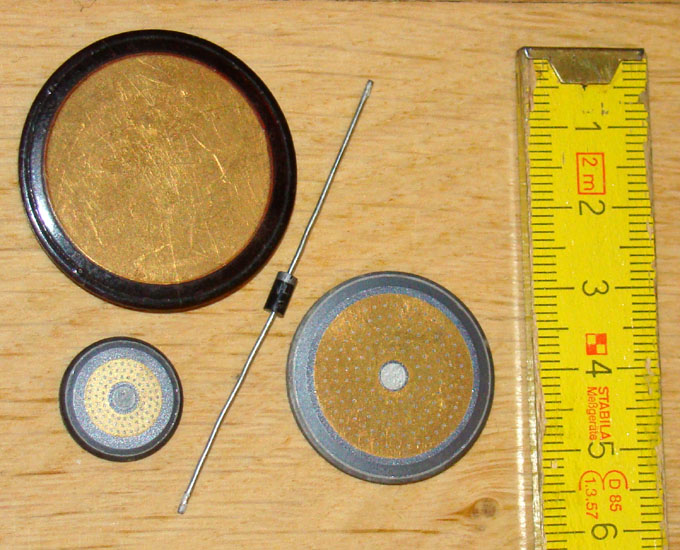
\includegraphics[height=0.45\textheight]{fig/lec05/Thyristor_example_01.jpg}
			\caption{Top left: \SI{1000}{\volt}/\SI{200}{\ampere} (diode); bottom left: \SI{1500}{\volt}/\SI{20}{\ampere}; right: \SI{1500}{\volt}/\SI{120}{\ampere}; 1N4007 (diode) (source: \href{https://de.wikipedia.org/wiki/Datei:SCR_power_rectifiers.jpg}{Wikimedia Commons}, \href{https://creativecommons.org/publicdomain/zero/1.0/}{CC0~1.0})}
        \end{subfigure}
        \hspace{1cm}
        \begin{subfigure}{0.45\textwidth}
            \centering
            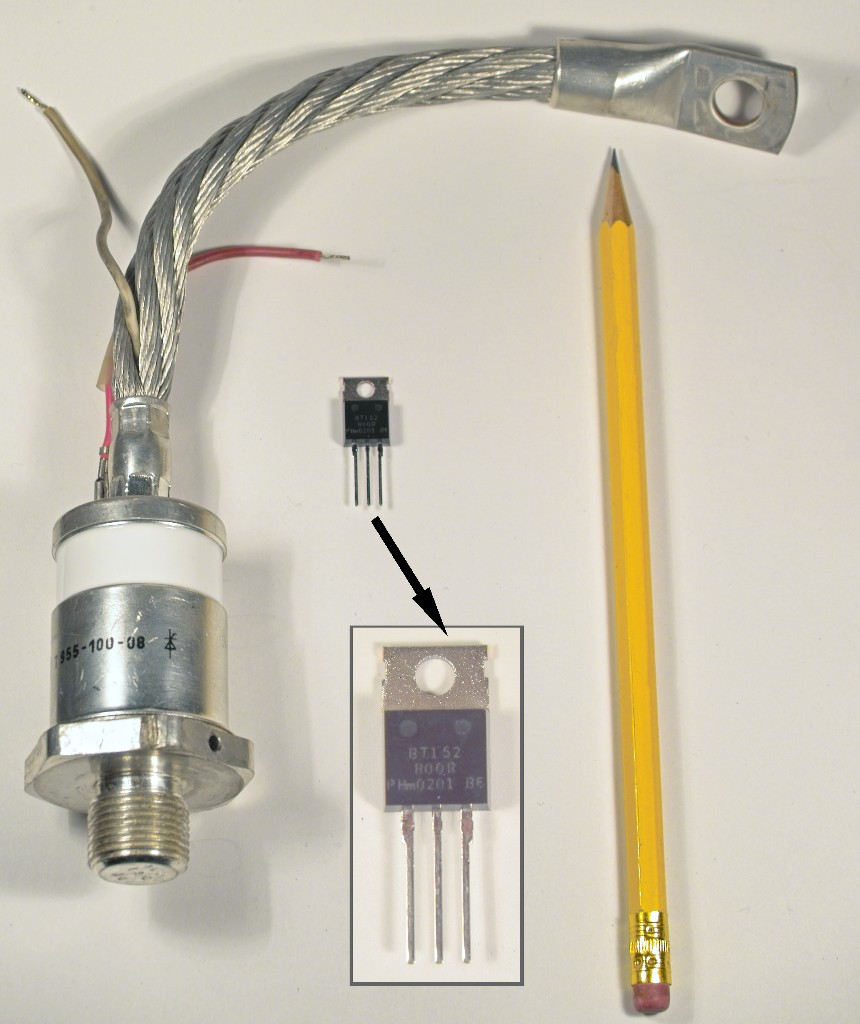
\includegraphics[height=0.45\textheight]{fig/lec05/Thyristor_example_02.jpg}
			\caption{Left: \SI{800}{\volt}/\SI{100}{\ampere}; right: \SI{800}{\volt}/\SI{13}{\ampere} (source: \href{https://de.wikipedia.org/wiki/Datei:Thyristors_thyristoren.jpg}{Wikimedia Commons}, Julo, \href{https://creativecommons.org/licenses/by-sa/3.0/deed.de}{CC0~BY-SA~3.0})}
            \vspace{1em}
        \end{subfigure}
        \caption{Thyristor examples with different voltage and current ratings}
        \label{fig:thyristor_examples}
    \end{figure}
\end{frame}

%%%%%%%%%%%%%%%%%%%%%%%%%%%%%%%%%%%%%%%%%%%%%%%%%%%%%%%%%%%%%
%% M1 rectifier comparison %%
%%%%%%%%%%%%%%%%%%%%%%%%%%%%%%%%%%%%%%%%%%%%%%%%%%%%%%%%%%%%%
\begin{frame}
    \frametitle{M1 rectifier comparison}
    \begin{columns}
        \begin{column}{0.5\textwidth}
            \centering
            \begin{circuitikz}[] % M1U diode circuit
                \draw (0,0) to [open, o-o, v = $u_1(t)\hspace{0.5cm}$, voltage = straight] ++(0,-1.5) coordinate (A)
                (0,0) to [short] ++(0.75,0)
                to [diode, l=$D$, v= $u_\mathrm{D}(t)$, voltage = straight]  ++(1.5,0)
                to [short, i=$i_2(t)$] ++(0.75,0)
                to [R, v^= $u_2(t)$, voltage = straight, l_=$R$] ++(0,-1.5) coordinate (B)
                (A) -- (B);
            \end{circuitikz}\\[1em]    
            \begin{tikzpicture}[] % M1U output voltage
                \begin{groupplot}[group style={group size=1 by 2, xticklabels at = edge bottom, vertical sep=1em}, 
                    width=0.85\textwidth,
                    height=0.31\textheight,
                    axis x line=bottom,
	                axis y line=left,
                    xmin=0, xmax=4*pi,
                    ymin=-0.01, ymax=1.15,
                    xtick={0,pi,2*pi, 3*pi, 4*pi},
                    xticklabels={$0$,$\pi$,$2\pi$,$3\pi$,$4\pi$},
                    ytick={-1,0,1},
                    yticklabels={$-\hat{u}_1$,$0$,$\hat{u}_1$},
                    grid=both,
                    ]
                \nextgroupplot[ylabel = {$u_2(\omega t)$}]
                    \addplot[domain=0:pi, samples=50, signalblue, thick, name path = A]{sin(deg(x))};
                    \addplot[domain=pi:2*pi, samples=10, signalblue, thick, name path = B]{0};
                    \addplot[domain=2*pi:3*pi, samples=50, signalblue, thick, name path = C]{sin(deg(x))};
                    \addplot[domain=3*pi:4*pi, samples=10, signalblue, thick, name path = D]{0};
                    \addplot[domain=0:4*pi, samples=10, signalblue, thick,dashed, name path = avg]{1/pi};
                    \node at (axis cs:3*pi/2,1/pi) [anchor=south] {$\overline{u}_2$};
                    \addplot[shadecolor, opacity=0.3] fill between[of=A and avg, soft clip={domain=0:pi}];
                    \addplot[shadecolor, opacity=0.3] fill between[of=B and avg, soft clip={domain=pi:2*pi}];
                    \addplot[shadecolor, opacity=0.3] fill between[of=C and avg, soft clip={domain=2*pi:3*pi}];
                    \addplot[shadecolor, opacity=0.3] fill between[of=D and avg, soft clip={domain=3*pi:4*pi}];

                \nextgroupplot[ylabel = {$u_\mathrm{D}(\omega t)$}, ymin=-1.15, ymax=1.15, height=0.4\textheight, xlabel = {$\omega t$}]
                    \addplot[domain=0:4*pi, samples=50, signalblue, dashed]{sin(deg(x))};
                    \addplot[domain=0:pi, samples=10, signalblue, thick]{0};
                    \addplot[domain=pi:2*pi, samples=50, signalblue, thick]{sin(deg(x))};
                    \addplot[domain=2*pi:3*pi, samples=10, signalblue, thick]{0};
                    \addplot[domain=3*pi:4*pi, samples=50, signalblue, thick]{sin(deg(x))};
                    \node at (axis cs:pi*3/4,1/pi) [anchor=south west] {${u}_1(\omega t)$};
                \end{groupplot}
            \end{tikzpicture}    
        \end{column}
        \begin{column}{0.5\textwidth}
            \centering
            \begin{circuitikz}[] % M1C thyristor circuit
                \draw (0,0) to [open, o-o, v = $u_1(t)\hspace{0.5cm}$, voltage = straight] ++(0,-1.5) coordinate (A)
                (0,0) to [short] ++(0.75,0)
                to [thyristor, voltage = straight, v= $u_\mathrm{T}(t)$, name = T]  ++(1.5,0)
                to [short, i=$i_2(t)$] ++(0.75,0)
                to [R, v^= $u_2(t)$, voltage = straight, l_=$R$] ++(0,-1.5) coordinate (B)
                (A) -- (B);
                \node at (T.gate) [above, xshift=-5mm, yshift=-2mm]{$T$};
            \end{circuitikz}\\[1em]    
            \begin{tikzpicture}[] % M1C output voltage
                \def\a{0.4*pi}
                \begin{groupplot}[group style={group size=1 by 2, xticklabels at = edge bottom, vertical sep=1em}, 
                    width=0.85\textwidth,
                    height=0.31\textheight,
                    axis x line=bottom,
	                axis y line=left,
                    xmin=0, xmax=4*pi,
                    ymin=-0.01, ymax=1.15,
                    xtick={0,pi,2*pi, 3*pi, 4*pi},
                    xticklabels={$0$,$\pi$,$2\pi$,$3\pi$,$4\pi$},
                    ytick={-1,0,1},
                    yticklabels={$-\hat{u}_1$,$0$,$\hat{u}_1$},
                    grid=both,
                    ]
                \nextgroupplot[ylabel = {$u_2(\omega t)$}]
                    \addplot[domain=0:2*pi, samples=150, signalblue, thick, name path = A]{max(sin(deg(x))*max(sign(x-\a),0),0)};
                    \addplot[domain=2*pi:4*pi, samples=150, signalblue, thick, name path = B]{max(sin(deg(x))*max(sign(x-\a-2*pi),0),0)};
                    \addplot[domain=0:4*pi, samples=10, signalblue, thick,dashed, name path = avg]{1/(2*pi)*(1+cos(deg(\a)))};
                    \node at (axis cs:3*pi/2,{1/(2*pi)*(1+cos(deg(\a)))}) [anchor=south] {$\overline{u}_2$};
                    \draw[->] (axis cs:0,0.5) -- node[above]{$\alpha$} (axis cs:\a,0.5) ;
                    \draw[->] (axis cs:2*pi,0.5) -- node[above]{$\alpha$} (axis cs:2*pi+\a,0.5) ;
                    \draw[dashed, thick] (axis cs:2*pi,0) -- (axis cs:2*pi,1);
                    \addplot[shadecolor, opacity=0.3] fill between[of=A and avg, soft clip={domain=0:2*pi}];
                    \addplot[shadecolor, opacity=0.3] fill between[of=B and avg, soft clip={domain=2*pi:4*pi}];


                \nextgroupplot[ylabel = {$u_\mathrm{T}(\omega t)$}, ymin=-1.15, ymax=1.15, height=0.4\textheight, xlabel = {$\omega t$}]
                    \addplot[domain=0:4*pi, samples=50, signalblue, dashed]{sin(deg(x))};
                    \addplot[domain=0:2*pi, samples=150, signalblue, thick]{max(sin(deg(x))*max(-sign(x-\a),0),0) + sin(deg(x))*max(sign(x-pi),0)};
                    \addplot[domain=2*pi:4*pi, samples=150, signalblue, thick]{max(sin(deg(x))*max(-sign(x-\a-2*pi),0),0) + sin(deg(x))*max(sign(x-3*pi),0)};
                    \node at (axis cs:pi*3/4,1/pi) [anchor=south west] {${u}_1(\omega t)$};
                \end{groupplot}
            \end{tikzpicture}          
        \end{column}
    \end{columns}
\end{frame}

%%%%%%%%%%%%%%%%%%%%%%%%%%%%%%%%%%%%%%%%%%%%%%%%%%%%%%%%%%%%%
%% Half-cycle rectification / M1C circuit %%
%%%%%%%%%%%%%%%%%%%%%%%%%%%%%%%%%%%%%%%%%%%%%%%%%%%%%%%%%%%%%
\subsection{M1C circuit} 

%%%%%%%%%%%%%%%%%%%%%%%%%%%%%%%%%%%%%%%%%%%%%%%%%%%%%%%%%%%%%
%% M1C rectifier %%
%%%%%%%%%%%%%%%%%%%%%%%%%%%%%%%%%%%%%%%%%%%%%%%%%%%%%%%%%%%%%
\begin{frame}
    \frametitle{M1C rectifier}
    \onslide<1->{The \hl{average output voltage} of the M1C circuit, i.e., the M1 rectifier with a thyristor, for a resistive load is given by}
    \begin{equation}
        \onslide<1->{\overline{u}_2 = \frac{1}{2\pi} \int_{\alpha}^{\pi} \hat{u}_1 \sin(\omega t) \mathrm{d} \omega t} \onslide<2->{= \frac{\hat{u}_1}{2\pi} \left[ -\cos(\omega t) \right]_{\alpha}^{\pi} = \frac{\hat{u}_1}{2\pi} \left( 1 + \cos(\alpha) \right).} 
    \end{equation}
    \onslide<2->{Here, $\alpha$ denotes the phase angle at which the thyristor is triggered (aka \hl{firing angle}).} \onslide<3->{In the M1C case, the \hl{feasible range} for $\alpha$ is $[0,\pi]$ as the thyristor requires a positive forward voltage to start conducting, that is, if $u_\mathrm{T}<0$ a firing impulse would not change its conduction state.} \onslide<4->{The \hl{RMS value} of the output voltage is given by}
    \begin{equation}
        \onslide<4->{ U_2 = \sqrt{\frac{1}{2\pi} \int_{\alpha}^{\pi} \hat{u}_1^2 \sin^2(\omega t) \mathrm{d} \omega t}}\onslide<5->{ =   \ldots = \frac{\hat{u}_1}{2} \sqrt{\frac{\pi - \alpha + \sin(\alpha)\cos(\alpha)}{\pi}}.}
    \end{equation}
    \onslide<6->{In contrast to the M1U rectifier from \eqref{eq:u2_M1U_avg}, the \hl{M1C rectifier allows for controlling the output voltage} by adjusting the firing angle $\alpha$.}
\end{frame}

%%%%%%%%%%%%%%%%%%%%%%%%%%%%%%%%%%%%%%%%%%%%%%%%%%%%%%%%%%%%%
%% M1C rectifier: Fourier series %%
%%%%%%%%%%%%%%%%%%%%%%%%%%%%%%%%%%%%%%%%%%%%%%%%%%%%%%%%%%%%%
\begin{frame}
    \frametitle{M1C rectifier: Fourier series}
    \onslide<1->{The \hl{Fourier coefficients} of the output voltage $u_2(t)$ for the M1C converter are}
    \begin{equation}
        \begin{split}
            \onslide<1->{a^{(0)} &= \frac{1}{\pi} \int_0^{2\pi} u_2(t) \mathrm{d} \omega t = \frac{1}{\pi} \int_{\alpha}^{\pi} \hat{u}_1 \sin(\omega t) \mathrm{d}\omega t} \onslide<2->{= 2 \overline{u}_2= \frac{\hat{u}_1}{\pi}(1+\cos(\alpha)),}\\
            \onslide<3->{a^{(k)} &= \frac{1}{\pi} \int_{0}^{2\pi} u_2(t) \cos(k\omega t) \mathrm{d}\omega t  = \frac{1}{\pi} \int_{\alpha}^{\pi} \hat{u}_1 \sin(\omega t) \cos(k\omega t) \mathrm{d}\omega t}\onslide<4->{=\ldots} \\ & \onslide<4->{=  \begin{cases}\frac{\hat{u}_1}{\pi}\frac{2}{1-k^2}, & k=1\\ \frac{1}{2\pi} \left( \frac{\cos(\alpha(k-1)) + \cos(k\pi)}{k-1} - \frac{\cos(\alpha(k+1)) + \cos(k\pi)}{k+1} \right), & k \geq 2. \end{cases} }\\
            \onslide<5->{b^{(k)} &= \frac{1}{\pi} \int_{0}^{2\pi} u_2(t) \sin(k\omega t) \mathrm{d}\omega t = \frac{1}{\pi} \int_{\alpha}^{\pi} \hat{u}_1 \sin(\omega t) \sin(k\omega t) \mathrm{d}\omega t}\onslide<6->{=\ldots} \\ &\onslide<6->{= \begin{cases} \frac{-\alpha + \pi + \cos(\alpha)\sin(\alpha)}{2\pi}, & k =1,\\ \frac{1}{2\pi} \left( \frac{\sin(\alpha(k-1)) + \sin(k\pi)}{k-1} - \frac{\sin(\alpha(k+1)) + \sin(k\pi)}{k+1} \right), & k \geq 2. \end{cases}}
        \end{split}
        \label{eq:u2_M1C_Fourier}
    \end{equation}
    \onslide<7->{In contrast to the M1U rectifier, one can observe additional harmonic components due to additional distortion of the output voltage caused by the thyristor switching.}
\end{frame}


%%%%%%%%%%%%%%%%%%%%%%%%%%%%%%%%%%%%%%%%%%%%%%%%%%%%%%%%%%%%%
%% M2C circuit %%
%%%%%%%%%%%%%%%%%%%%%%%%%%%%%%%%%%%%%%%%%%%%%%%%%%%%%%%%%%%%%
\subsection{M2C circuit} 

%%%%%%%%%%%%%%%%%%%%%%%%%%%%%%%%%%%%%%%%%%%%%%%%%%%%%%%%%%%%%
%% M2C controllable rectifier circuit  %%
%%%%%%%%%%%%%%%%%%%%%%%%%%%%%%%%%%%%%%%%%%%%%%%%%%%%%%%%%%%%%
\begin{frame}[c]
    \frametitle{M2C converter}
    \begin{figure}
           \begin{circuitikz}[baseline=(current bounding box.center)]
            \draw (0,0) node[transformer core](T){$N_1:N_2$}
            (T.inner dot A1) node[circ]{}
            (T.inner dot B1) node[circ]{}
            (T.A1) to [short] ++(0,1) to [short, -o, i<_=$i_1(t)$] ++(-1,0) coordinate (A1)
            (T.A2) to [short] ++(0,-1) to [short, -o] ++(-1,0) coordinate (A2)
            (T.B1) to [short] ++(0, 1) coordinate (B1)
            (T.B2) to [short] ++(0,-1) coordinate (B2);
            \draw (A1) to [open, v=$u_1(t)\hspace{0.5cm}$, voltage = straight] (A2); 
            \draw (B1) to [thyristor, name=T1] ++(2.0,0) coordinate (C1)
            (B2) to [thyristor, name=T2] ++(2.0,0)
            to [crossing, -*, mirror] (C1)
            to [short, i=$i_2(t)$] ++(1.0,0) coordinate (D)
            to [R, v^= $u_2(t)$, voltage = straight, l_=$R$] (T-L2.midtap -| D)
            to [short] (T-L2.midtap);
            \draw let \p1 = (B1), \p2 = (T-L2.midtap) in (\x1 + 0.5cm, \y1) to [open, v^=$\hspace{0.5cm}{u_\mathrm{s,1}(t)}$, voltage = straight] (\x1 + 0.5cm, \y2);
            \draw let \p1 = (B2), \p2 = (T-L2.midtap) in (\x1 + 0.5cm, \y1) to [open, v=$\hspace{0.5cm}{u_\mathrm{s,2}(t)}$, voltage = straight] (\x1 + 0.5cm, \y2);
            \node at (T1.gate) [above, xshift=-5mm, yshift=-2mm]{$T_1$};
            \node at (T2.gate) [below, xshift=-5mm, yshift=-7mm]{$T_2$};
        \end{circuitikz}%
        \hspace{0.25cm}
        \begin{tikzpicture}[baseline=(current bounding box.center)] % M1C output voltage
            \def\a{0.4*pi}
            \begin{groupplot}[group style={group size=1 by 2, xticklabels at = edge bottom, vertical sep=1em}, 
                width=0.38\textwidth,
                height=0.4\textheight,
                axis x line=bottom,
                axis y line=left,
                xmin=0, xmax=4*pi,
                ymin=-1.15, ymax=1.15,
                xtick={0,pi,2*pi, 3*pi, 4*pi},
                xticklabels={$0$,$\pi$,$2\pi$,$3\pi$,$4\pi$},
                ytick={-1,0,1},
                yticklabels={$-\hat{u}_\mathrm{s}$,$0$,$\hat{u}_\mathrm{s}$},
                grid=both,
                clip=false
                ]
            \nextgroupplot[ylabel = {$u_2(\omega t)$}]
                \addplot[domain=0:pi, samples=50, signalblue, thick, name path = A]{(x < \a) * 0 + (x > \a) * sin(deg(x))};
                \addplot[domain=pi:2*pi, samples=50, signalblue, thick, name path = B]{(x - pi < \a) * 0 + (x - pi > \a) * -sin(deg(x))};
                \addplot[domain=2*pi:3*pi, samples=50, signalblue, thick, name path = C]{(x - 2*pi < \a) * 0 + (x - 2*pi > \a) * sin(deg(x))};
                \addplot[domain=3*pi:4*pi, samples=50, signalblue, thick, name path = D]{(x - 3*pi < \a) * 0 + (x - 3*pi > \a) * -sin(deg(x))};
                \addplot[domain=0:4*pi, samples=10, signalblue, thick,dashed, name path = avg]{1/(pi)*(1+cos(deg(\a)))};
                \node at (axis cs:3*pi/2+0.4,{1/(pi)*(1+cos(deg(\a)))}) [anchor=north] {$\overline{u}_2$};
                \draw[->] (axis cs:0,1) -- node[above]{$\alpha$} (axis cs:\a,1) ;
                \draw[->] (axis cs:2*pi,1) -- node[above]{$\alpha$} (axis cs:2*pi+\a,1) ;
                \draw[dashed, thick] (axis cs:2*pi,0) -- (axis cs:2*pi,1);
                \addplot[domain=0:4*pi, samples=50, signalgreen, dashed]{sin(deg(x))};
                \addplot[domain=0:4*pi, samples=50, signalbrown, dashed]{-sin(deg(x))};
                \node at (axis cs:pi*2.5,-0.75) [anchor=south, signalbrown] {$u_{s,2}$};
                \node at (axis cs:pi*3.5,-0.75) [anchor=south, signalgreen] {$u_{s,1}$};
                \addplot[shadecolor, opacity=0.3] fill between[of=A and avg, soft clip={domain=0:pi}];
                \addplot[shadecolor, opacity=0.3] fill between[of=B and avg, soft clip={domain=pi:2*pi}];
                \addplot[shadecolor, opacity=0.3] fill between[of=C and avg, soft clip={domain=2*pi:3*pi}];
                \addplot[shadecolor, opacity=0.3] fill between[of=D and avg, soft clip={domain=3*pi:4*pi}];


            \nextgroupplot[ylabel = {$u_\mathrm{T}(\omega t)$}, xlabel = {$\omega t$}, ymin=-2.15, ytick={-2, -1,0,1}, yticklabels={$-2\hat{u}_\mathrm{s}$, $-\hat{u}_\mathrm{s}$,$0$,$\hat{u}_\mathrm{s}$}, height=0.5\textheight]
                \node at (axis cs:\a,0.5) [signalgreen, right, inner sep=1pt] {${u}_{T_1}$};
                \node at (axis cs:\a+pi,0.5) [signalbrown, right, inner sep=1pt] {${u}_{T_2}$};
                \addplot[domain=0:pi, samples=50, signalgreen, thick]{(x < \a) * sin(deg(x)) + (x > \a) * 0};
                \addplot[domain=0:pi, samples=50, signalbrown, thick]{-sin(deg(x)) + (x > \a) * -sin(deg(x))};
                \addplot[domain=pi:2*pi, samples=50, signalbrown, thick]{(x -pi < \a) * -sin(deg(x)) + (x-pi > \a) * 0};
                \addplot[domain=pi:2*pi, samples=50, signalgreen, thick]{sin(deg(x)) + (x -pi > \a) * sin(deg(x))};
                \addplot[domain=2*pi:3*pi, samples=50, signalgreen, thick]{(x -2*pi < \a) * sin(deg(x)) + (x  -2*pi > \a) * 0};
                \addplot[domain=2*pi:3*pi, samples=50, signalbrown, thick]{-sin(deg(x)) + (x  -2*pi > \a) * -sin(deg(x))};
                \addplot[domain=3*pi:4*pi, samples=50, signalbrown, thick]{(x - 3*pi < \a) * -sin(deg(x)) + (x - 3*pi > \a) * 0};
                \addplot[domain=3*pi:4*pi, samples=50, signalgreen, thick]{sin(deg(x)) + (x - 3*pi > \a) * sin(deg(x))};
            \end{groupplot}
        \end{tikzpicture}   
        \caption{M2C topology (aka \hl{two-pulse mid-point converter}) with center-tapped transformer and a resistive load}
        \label{fig:M2C_topology}
    \end{figure}
\end{frame}

%%%%%%%%%%%%%%%%%%%%%%%%%%%%%%%%%%%%%%%%%%%%%%%%%%%%%%%%%%%%%
%% M2C converter: resistive load  %%
%%%%%%%%%%%%%%%%%%%%%%%%%%%%%%%%%%%%%%%%%%%%%%%%%%%%%%%%%%%%%
\begin{frame}
    \frametitle{M2C converter: resistive load}
    \onslide<1->{The \hl{average output voltage} of the M2C converter for a resistive load is given by}
    \begin{equation}
        \onslide<1->{\overline{u}_2 = \frac{1}{\pi} \int_{\alpha}^{\pi} \hat{u}_\mathrm{s} \sin(\omega t) \mathrm{d} \omega t} \onslide<2->{= \frac{\hat{u}_\mathrm{s}}{\pi} \left[ -\cos(\omega t) \right]_{\alpha}^{\pi} = \frac{\hat{u}_\mathrm{s}}{\pi} \left( 1 + \cos(\alpha) \right).}
    \end{equation}
    \onslide<3->{The \hl{RMS value} of the output voltage results in}
    \begin{equation}
        \onslide<3->{U_2 = \sqrt{\frac{1}{\pi} \int_{\alpha}^{\pi} \hat{u}_\mathrm{s}^2 \sin^2(\omega t) \mathrm{d} \omega t}} \onslide<4->{=   \ldots = \frac{\hat{u}_\mathrm{s}}{\sqrt{2}} \sqrt{\frac{\pi - \alpha + \sin(\alpha)\cos(\alpha)}{\pi}}.}
    \end{equation}
    \onslide<5->{The primary to secondary voltage ratio of the center-tapped transformer yields
    \begin{equation*}
        \frac{\hat{u}_\mathrm{s}}{\hat{u}_1} = \frac{1}{2}\frac{N_2}{N_1}.
    \end{equation*}}%
    \onslide<6->{It should be noted that in the case of a resistive load, the M2C's output voltage is always positive for the feasible firing angle range $\alpha \in [0,\pi]$.}
\end{frame}

%%%%%%%%%%%%%%%%%%%%%%%%%%%%%%%%%%%%%%%%%%%%%%%%%%%%%%%%%%%%%
%% M2C converter with an output filter  %%
%%%%%%%%%%%%%%%%%%%%%%%%%%%%%%%%%%%%%%%%%%%%%%%%%%%%%%%%%%%%%
\begin{frame}[c]
    \frametitle{M2C converter with an output filter}
    \begin{figure}
           \begin{circuitikz}[baseline=(current bounding box.center)]
            \draw (0,0) node[transformer core](T){$N_1:N_2$}
            (T.inner dot A1) node[circ]{}
            (T.inner dot B1) node[circ]{}
            (T.A1) to [short] ++(0,1) to [short, -o, i<_=$i_1(t)$] ++(-1,0) coordinate (A1)
            (T.A2) to [short] ++(0,-1) to [short, -o] ++(-1,0) coordinate (A2)
            (T.B1) to [short] ++(0, 1) coordinate (B1)
            (T.B2) to [short] ++(0,-1) coordinate (B2);
            \draw (A1) to [open, v=$u_1(t)\hspace{0.5cm}$, voltage = straight] (A2); 
            \draw (B1) to [thyristor, name=T1] ++(2.0,0) coordinate (C1)
            (B2) to [thyristor, name=T2] ++(2.0,0)
            to [crossing, -*, mirror] (C1)
            to [short] ++(0.5,0) coordinate (us)
            to [L, l=$L$] ++(2,0) 
            to [short] ++(0.5,0) coordinate (D)
            to [short, i=$i_2(t)$] ++(1.5,0)
            to [open, v^= $\hspace{0.5cm}u_2(t)$, voltage = straight, o-o] (T-L2.midtap -| \tikztostart)
            to [short] (\tikztostart -| D)
            (D) to [C, voltage = straight, l=$C$, *-*] (T-L2.midtap -| D)
            to [short] (T-L2.midtap);
            \draw (us) to [open, v^=$\hspace{0.5cm}u_\mathrm{s}(t)$, voltage = straight] (T-L2.midtap -| us);
            \draw let \p1 = (B1), \p2 = (T-L2.midtap) in (\x1 + 0.5cm, \y1) to [open, v^=$\hspace{0.5cm}{u_\mathrm{s,1}(t)}$, voltage = straight] (\x1 + 0.5cm, \y2);
            \draw let \p1 = (B2), \p2 = (T-L2.midtap) in (\x1 + 0.5cm, \y1) to [open, v=$\hspace{0.5cm}{u_\mathrm{s,2}(t)}$, voltage = straight] (\x1 + 0.5cm, \y2);
            \node at (T1.gate) [above, xshift=-5mm, yshift=-2mm]{$T_1$};
            \node at (T2.gate) [below, xshift=-5mm, yshift=-7mm]{$T_2$};
        \end{circuitikz}%
        \caption{M2C converter with an output filter assuming $u_2(t)=U_2=\mbox{const.}$}
        \label{fig:M2C_output_filter}
    \end{figure}
\end{frame}

%%%%%%%%%%%%%%%%%%%%%%%%%%%%%%%%%%%%%%%%%%%%%%%%%%%%%%%%%%%%%
%% M2C converter with an output filter  %%
%%%%%%%%%%%%%%%%%%%%%%%%%%%%%%%%%%%%%%%%%%%%%%%%%%%%%%%%%%%%%
\begin{frame}[c]
    \frametitle{M2C converter with an output filter (cont.)}
    \begin{figure}
        \begin{tikzpicture} % M1C output voltage
            \tikzmath{
                    real \a, \iLavg1, \iLavg1, \Lw, \u1, \uc1, \iLs1, \iLs2, \b, \adcm;
                    \a = 0.3*pi; %firing angle
                    \Lw = 2; %angular frequency times inductance
                    \u1 = 1; %Input voltage amplitude
                    \uc1 = 2*\u1/pi*cos(deg(\a)); %output voltage for CCM
                    \iLs1 = 0.6; %current initial value for CCM
                    \iLs2 = -1/\Lw*(-\uc1*\a + \u1*(cos(deg(\a))-1)); %current initial value for BCM
                    \iLavg1 = \iLs1 + 1/(\Lw*pi)*(-\uc1*(pi^2/2) + \u1*(2*sin(deg(\a)) - \a + (2*cos(deg(\a))-1)*(pi-\a))); %current average value for CCM
                    \iLavg2 = \iLs2 + 1/(\Lw*pi)*(-\uc1*(pi^2/2) + \u1*(2*sin(deg(\a)) - \a + (2*cos(deg(\a))-1)*(pi-\a))); %current average value for BCM
                    \b = 0.8*pi; %conduction interval for DCM
                    \adcm = 0.4*pi; %firing angle for DCM (\b + \adcm must be greater than pi for corret visualization)
                    \ucdcm = -1/\b*(\u1*(cos(deg(\adcm+\b))-cos(deg(\adcm)))); %output voltage for DCM
                    \iLavg3 = 1/(\Lw*pi)*(-\u1*(sin(deg(\adcm+\b))-sin(deg(\adcm))-cos(deg(\adcm))*\b) - \ucdcm*(\b^2/2)); %current average value for DCM
                }
            \begin{groupplot}[group style={group size=3 by 2, xticklabels at = edge bottom, vertical sep=1em, yticklabels at = edge left, horizontal sep = 1em}, 
                width=0.38\textwidth,
                height=0.34\textheight,
                axis x line=bottom,
                axis y line=left,
                xmin=0, xmax=2*pi,
                ymin=-1.15, ymax=1.15,
                xtick={0, pi/2, pi, 3*pi/2, 2*pi},
                xticklabels={$0$,$\frac{1}{2}\pi$, $\pi$,$\frac{3}{2}\pi$, $2\pi$},
                ytick={-1, -1/2, 0,1/2, 1},
                yticklabels={$-\hat{u}_\mathrm{s}$, ,$0$, ,$\hat{u}_\mathrm{s}$},
                grid=both,
                clip=false
                ]
            \nextgroupplot[ylabel = {$u_\mathrm{s}(\omega t)$}, title=CCM, height=0.475\textheight] % voltage CCM
                \addplot[domain=0:pi, samples=50, signalblue, thick, name path = A1]{(x < \a) * -sin(deg(x)) + (x > \a) * sin(deg(x))};
                \addplot[domain=pi:2*pi, samples=50, signalblue, thick, name path = B1]{(x - pi < \a) * sin(deg(x)) + (x - pi > \a) * -sin(deg(x))};
                \addplot[domain=0:2*pi, samples=10, signalblue, thick,dashed, name path = avg1]{2/(pi)*(cos(deg(\a)))};
                \node at (axis cs:3*pi/2+0.4,{2/(pi)*(cos(deg(\a)))}) [anchor=north] {$\overline{u}_2$};
                \draw[->] (axis cs:0,1) -- node[above]{$\alpha$} (axis cs:\a,1) ;
                \draw[->] (axis cs:pi,1) -- node[above]{$\alpha$} (axis cs:pi+\a,1) ;
                \draw[dashed, thick] (axis cs:pi,0) -- (axis cs:pi,1);
                \addplot[domain=0:2*pi, samples=50, signalgreen, dashed]{sin(deg(x))};
                \addplot[domain=0:2*pi, samples=50, signalbrown, dashed]{-sin(deg(x))};
                \node at (axis cs:pi*3/4,-0.75) [signalbrown, fill=white,inner sep=1pt] {$u_{s,2}$};
                \node at (axis cs:pi*7/4,-0.75) [signalgreen, fill=white,inner sep=1pt] {$u_{s,1}$};
                \addplot[shadecolor, opacity=0.3] fill between[of=A1 and avg1, soft clip={domain=0:pi}];
                \addplot[shadecolor, opacity=0.3] fill between[of=B1 and avg1, soft clip={domain=pi:2*pi}];

            \nextgroupplot[title=BCM, height=0.475\textheight, visible on=<2->] % voltage BCM
                \addplot[domain=0:pi, samples=50, signalblue, thick, name path = A2]{(x < \a) * -sin(deg(x)) + (x > \a) * sin(deg(x))};
                \addplot[domain=pi:2*pi, samples=50, signalblue, thick, name path = B2]{(x - pi < \a) * sin(deg(x)) + (x - pi > \a) * -sin(deg(x))};
                \addplot[domain=0:2*pi, samples=10, signalblue, thick,dashed, name path = avg2]{2/(pi)*(cos(deg(\a)))};
                \node at (axis cs:3*pi/2+0.4,{2/(pi)*(cos(deg(\a)))}) [anchor=north] {$\overline{u}_2$};
                \draw[->] (axis cs:0,1) -- node[above]{$\alpha$} (axis cs:\a,1) ;
                \draw[->] (axis cs:pi,1) -- node[above]{$\alpha$} (axis cs:pi+\a,1) ;
                \draw[dashed, thick] (axis cs:pi,0) -- (axis cs:pi,1);
                \addplot[domain=0:2*pi, samples=50, signalgreen, dashed]{sin(deg(x))};
                \addplot[domain=0:2*pi, samples=50, signalbrown, dashed]{-sin(deg(x))};
                \node at (axis cs:pi*3/4,-0.75) [signalbrown, fill=white,inner sep=1pt] {$u_{s,2}$};
                \node at (axis cs:pi*7/4,-0.75) [signalgreen, fill=white,inner sep=1pt] {$u_{s,1}$};
                \addplot[shadecolor, opacity=0.3, visible on=<2->] fill between[of=A2 and avg2, soft clip={domain=0:pi}];
                \addplot[shadecolor, opacity=0.3, visible on=<2->] fill between[of=B2 and avg2, soft clip={domain=pi:2*pi}];

            \nextgroupplot[title=DCM, height=0.475\textheight, visible on=<3->] % voltage DCM
                \addplot[domain=0:2*pi, samples=200, signalblue, thick, name path = A3]{(x < \adcm +\b - pi) * sin(deg(x+pi)) + (x > \adcm + \b -pi) * (x < \adcm) * \ucdcm + (x > \adcm)* (x < \adcm + \b) * sin(deg(x)) + (x > \adcm + \b) * (x < \adcm + pi) * \ucdcm + (x > \adcm + pi) * sin(deg(x-pi))};
                \addplot[domain=0:2*pi, samples=10, signalblue, thick,dashed, name path = avg3]{\ucdcm};
                \node at (axis cs:3*pi/2+0.4,\ucdcm) [anchor=north] {$\overline{u}_2$};
                \addplot[domain=0:2*pi, samples=50, signalgreen, dashed]{sin(deg(x))};
                \addplot[domain=0:2*pi, samples=50, signalbrown, dashed]{-sin(deg(x))};
                \node at (axis cs:pi*3/4,-0.75) [signalbrown, fill=white,inner sep=1pt] {$u_{s,2}$};
                \node at (axis cs:pi*7/4,-0.75) [signalgreen, fill=white,inner sep=1pt] {$u_{s,1}$};
                \draw[->] (axis cs:0,1) -- node[above]{$\alpha$} (axis cs:\adcm,1) ;
                \draw[->] (axis cs:pi,1) -- node[above]{$\alpha$} (axis cs:pi+\adcm,1) ;
                \draw[dashed, thick] (axis cs:pi,0) -- (axis cs:pi,1);
                \addplot[shadecolor, opacity=0.3, visible on=<3->] fill between[of=A3 and avg3, soft clip={domain=0:2*pi}];
                


            \nextgroupplot[ylabel = {$i_\mathrm{L}(\omega t)$}, xlabel = {$\omega t$}, ymin=-0.01, ytick={0, 1/2, 1}, yticklabels={$0$, } ] %current CCM
                \addplot[domain=0:\a, samples=50, signalred, thick, name path = Ai1]{1/\Lw*(-\uc1*x + \u1*(cos(deg(x))-1))+\iLs1};
                \addplot[domain=\a:pi, samples=50, signalred, thick, name path = Bi1]{1/\Lw*(-\uc1*\a + \u1*(cos(deg(\a))-1))+\iLs1 + 1/\Lw*(\u1*(-cos(deg(x))+cos(deg(\a))) - \uc1*(x-\a))};
                \addplot[domain=pi:pi+\a, samples=50, signalred, thick, name path = Ci1]{1/\Lw*(-\uc1*(x-pi) + \u1*(cos(deg(x - pi))-1))+\iLs1};
                \addplot[domain=pi+\a:2*pi, samples=50, signalred, thick, name path = Di1]{1/\Lw*(-\uc1*\a + \u1*(cos(deg(\a))-1))+\iLs1 + 1/\Lw*(\u1*(-cos(deg(x-pi))+cos(deg(\a))) - \uc1*(x-\a-pi))};
                \addplot[domain=0:2*pi, samples=10, signalred, thick,dashed, name path = avgi1]{\iLavg1};
                \draw[<->] (axis cs:\a,0.75) -- node[above, fill = white]{$\beta=\pi$} (axis cs:\a+pi,0.75) ;
                \addplot[shadecolor, opacity=0.3] fill between[of=Ai1 and avgi1, soft clip={domain=0:\a}];
                \addplot[shadecolor, opacity=0.3] fill between[of=Bi1 and avgi1, soft clip={domain=\a:pi}];
                \addplot[shadecolor, opacity=0.3] fill between[of=Ci1 and avgi1, soft clip={domain=pi:pi+\a}];
                \addplot[shadecolor, opacity=0.3] fill between[of=Di1 and avgi1, soft clip={domain=pi+\a:2*pi}];

            \nextgroupplot[xlabel = {$\omega t$}, ymin=-0.01, ytick={0, 1/2, 1}, yticklabels={ } , visible on=<2->] %current BCM
                \addplot[domain=0:\a, samples=50, signalred, thick, name path = Ai2]{1/\Lw*(-\uc1*x + \u1*(cos(deg(x))-1))+\iLs2};
                \addplot[domain=\a:pi, samples=50, signalred, thick, name path = Bi2]{1/\Lw*(-\uc1*\a + \u1*(cos(deg(\a))-1))+\iLs2 + 1/\Lw*(\u1*(-cos(deg(x))+cos(deg(\a))) - \uc1*(x-\a))};
                \addplot[domain=pi:pi+\a, samples=50, signalred, thick, name path = Ci2]{1/\Lw*(-\uc1*(x-pi) + \u1*(cos(deg(x - pi))-1))+\iLs2};
                \addplot[domain=pi+\a:2*pi, samples=50, signalred, thick, name path = Di2]{1/\Lw*(-\uc1*\a + \u1*(cos(deg(\a))-1))+\iLs2 + 1/\Lw*(\u1*(-cos(deg(x-pi))+cos(deg(\a))) - \uc1*(x-\a-pi))};
                \addplot[domain=0:2*pi, samples=10, signalred, thick,dashed, name path = avgi2]{\iLavg2};
                \draw[<->] (axis cs:\a,0.6) -- node[above, fill = white]{$\beta=\pi$} (axis cs:\a+pi,0.6) ;
                \addplot[shadecolor, opacity=0.3, visible on=<2->] fill between[of=Ai2 and avgi2, soft clip={domain=0:\a}];
                \addplot[shadecolor, opacity=0.3, visible on=<2->] fill between[of=Bi2 and avgi2, soft clip={domain=\a:pi}];
                \addplot[shadecolor, opacity=0.3, visible on=<2->] fill between[of=Ci2 and avgi2, soft clip={domain=pi:pi+\a}];
                \addplot[shadecolor, opacity=0.3, visible on=<2->] fill between[of=Di2 and avgi2, soft clip={domain=pi+\a:2*pi}];

            \nextgroupplot[xlabel = {$\omega t$}, ymin=-0.01, ytick={0, 1/2, 1}, yticklabels={}, visible on=<3->] %current DCM
                \addplot[domain=\adcm:\adcm+\b, samples=50, signalred, thick, name path = Ai3]{1/\Lw*(-\ucdcm*(x-\adcm) - \u1*(cos(deg(x))-cos(deg(\adcm))))};
                \addplot[domain=0:\adcm+\b-pi, samples=50, signalred, thick, name path = Bi3]{1/\Lw*(-\ucdcm*(x-\adcm+pi) - \u1*(cos(deg(x+pi))-cos(deg(\adcm))))};
                \addplot[domain=\adcm+pi:2*pi, samples=50, signalred, thick, name path = Ci3]{1/\Lw*(-\ucdcm*(x-\adcm-pi) - \u1*(cos(deg(x-pi))-cos(deg(\adcm))))};
                \addplot[domain=\adcm+\b:\adcm+pi, samples=50, signalred, thick, name path = Di3]{0};
                \addplot[domain=\adcm+\b-pi:\adcm, samples=50, signalred, thick, name path = Ei3]{0};
                \addplot[domain=0:2*pi, samples=10, signalred, thick,dashed, name path = avgi3]{\iLavg3};
                \draw[<->] (axis cs:\adcm,0.5) -- node[above, fill = white]{$\beta<\pi$} (axis cs:\adcm+\b,0.5) ;
                \addplot[shadecolor, opacity=0.3, visible on=<3->] fill between[of=Ai3 and avgi3, soft clip={domain=\adcm:\adcm+\b}];
                \addplot[shadecolor, opacity=0.3, visible on=<3->] fill between[of=Bi3 and avgi3, soft clip={domain=0:\adcm+\b-pi}];
                \addplot[shadecolor, opacity=0.3, visible on=<3->] fill between[of=Ci3 and avgi3, soft clip={domain=\adcm+pi:2*pi}];
                \addplot[shadecolor, opacity=0.3, visible on=<3->] fill between[of=Di3 and avgi3, soft clip={domain=\adcm+\b:\adcm+pi}];
                \addplot[shadecolor, opacity=0.3, visible on=<3->] fill between[of=Ei3 and avgi3, soft clip={domain=\adcm+\b-pi:\adcm}];

            \end{groupplot}
        \end{tikzpicture}   
        \caption{M2C topology with an output filter and different average load currents}
        \label{fig:M2C_different_loads}
    \end{figure}
\end{frame}

%%%%%%%%%%%%%%%%%%%%%%%%%%%%%%%%%%%%%%%%%%%%%%%%%%%%%%%%%%%%%
%% M2C converter with an output filter  %%
%%%%%%%%%%%%%%%%%%%%%%%%%%%%%%%%%%%%%%%%%%%%%%%%%%%%%%%%%%%%%
\begin{frame}[c]
    \frametitle{M2C converter with an output filter (cont.)}
    \onslide<1->{Due to the output filter, the secondary voltage $u_\mathrm{s}(t)$ can become negative since the current flow is maintained by the inductor and, therefore, a thyristor is remaining in the conducting state (until the next thyristor is triggered). The \hl{average output voltage in CCM (and BCM)} is given by}
    \begin{equation}
        \begin{split}
            \onslide<1->{\overline{u}_2 &= \frac{1}{\pi} \int_{\alpha}^{\alpha+\pi} \hat{u}_\mathrm{s} \sin(\omega t) \mathrm{d} \omega t} \onslide<2->{= \frac{\hat{u}_\mathrm{s}}{\pi} \left[ -\cos(\omega t) \right]_{\alpha}^{\alpha+\pi} = \frac{\hat{u}_\mathrm{s}}{\pi} \left(-\cos(\alpha+\pi) +\cos(\alpha)\right)\\
             &= \hat{u}_\mathrm{s}\frac{2}{\pi} \cos(\alpha).}
        \end{split}
        \label{eq:u2_avg_M2C_CCM}
    \end{equation}
    \onslide<3->{In \hl{DCM} the \hl{conduction interval} $\beta$ is less than $\pi$ and the \hl{average output voltage} is given by}
    \begin{equation}
        \begin{split}
            \onslide<3->{\overline{u}_2 &= \frac{1}{\pi} \int_{\alpha}^{\alpha+\beta} \hat{u}_\mathrm{s} \sin(\omega t) \mathrm{d} \omega t} \onslide<4->{= \frac{\hat{u}_\mathrm{s}}{\pi} \left[ -\cos(\omega t) \right]_{\alpha}^{\alpha+\beta} = \frac{\hat{u}_\mathrm{s}}{\pi} \left(\cos(\alpha)-\cos(\alpha+\beta)\right)}\\
                \onslide<5->{ &= \hat{u}_\mathrm{s}\frac{2}{\pi}\sin\left(\frac{\beta}{2}\right)\sin\left(\alpha + \frac{\beta}{2}\right).}
    \end{split}
    \end{equation}
\end{frame}

%%%%%%%%%%%%%%%%%%%%%%%%%%%%%%%%%%%%%%%%%%%%%%%%%%%%%%%%%%%%%
%% M2C converter with an active load  %%
%%%%%%%%%%%%%%%%%%%%%%%%%%%%%%%%%%%%%%%%%%%%%%%%%%%%%%%%%%%%%
\begin{frame}[c]
    \frametitle{M2C converter with an active load}
    \onslide<1->{Analyzing \eqref{eq:u2_avg_M2C_CCM} for the feasible firing angle range $\alpha \in [0,\pi]$ reveals
    \begin{equation}
        \overline{u}_2 \begin{cases}
            \geq 0, & \alpha \in [0,\pi/2],\\
            < 0, & \alpha \in (\pi/2,\pi],
        \end{cases}
    \end{equation}
    that is, the \hl{output voltage can become negative} for $\alpha > \pi/2$ in CCM and BCM (analogous observation can be also made for DCM).}\onslide<2->{ Assuming an average output current $\overline{i}_{2} > 0$, which can be only positive due to the thyristor unipolar current capability, the \hl{average output power} is in the range of (for CCM and BCM) 
    \begin{equation}
        \overline{p}_2 \begin{cases}
            \geq 0, & \alpha \in [0,\pi/2],\\
            < 0, & \alpha \in (\pi/2,\pi].
        \end{cases}
    \end{equation}}
    \onslide<3->{Hence, the M2C can transfer energy from the load to the source which requires an active load (e.g., battery or generator) to maintain this reversed energy flow. Consequently, the M2C can be used as a \hl{bidirectional energy transfer system} operating both as a \hl{rectifier} and an \hl{inverter}.}
\end{frame}

%%%%%%%%%%%%%%%%%%%%%%%%%%%%%%%%%%%%%%%%%%%%%%%%%%%%%%%%%%%%%
%% M2C converter with an active load (cont.) %%
%%%%%%%%%%%%%%%%%%%%%%%%%%%%%%%%%%%%%%%%%%%%%%%%%%%%%%%%%%%%%
\begin{frame}[c]
    \frametitle{M2C converter with an active load (cont.)}
    \begin{figure}
        \begin{tikzpicture} % M1C output voltage
            \tikzmath{
                    real \a, \iLavg1, \iLavg1, \Lw, \u1, \uc1, \iLs1, \iLs2, \b, \adcm;
                    \a = 0.8*pi; %firing angle
                    \Lw = 2; %angular frequency times inductance
                    \u1 = 1; %Input voltage amplitude
                    \uc1 = 2*\u1/pi*cos(deg(\a)); %output voltage for CCM
                    \iLs1 = 0.6; %current initial value for CCM
                    \iLs2 = -1/\Lw*(-\uc1*\a + \u1*(cos(deg(\a))-1)); %current initial value for BCM
                    \iLavg1 = \iLs1 + 1/(\Lw*pi)*(-\uc1*(pi^2/2) + \u1*(2*sin(deg(\a)) - \a + (2*cos(deg(\a))-1)*(pi-\a))); %current average value for CCM
                    \iLavg2 = \iLs2 + 1/(\Lw*pi)*(-\uc1*(pi^2/2) + \u1*(2*sin(deg(\a)) - \a + (2*cos(deg(\a))-1)*(pi-\a))); %current average value for BCM
                    \b = 0.8*pi; %conduction interval for DCM
                    \adcm = 0.8*pi; %firing angle for DCM (\b + \adcm must be greater than pi for corret visualization)
                    \ucdcm = -1/\b*(\u1*(cos(deg(\adcm+\b))-cos(deg(\adcm)))); %output voltage for DCM
                    \iLavg3 = 1/(\Lw*pi)*(-\u1*(sin(deg(\adcm+\b))-sin(deg(\adcm))-cos(deg(\adcm))*\b) - \ucdcm*(\b^2/2)); %current average value for DCM
                }
            \begin{groupplot}[group style={group size=3 by 2, xticklabels at = edge bottom, vertical sep=1em, yticklabels at = edge left, horizontal sep = 1em}, 
                width=0.38\textwidth,
                height=0.34\textheight,
                axis x line=bottom,
                axis y line=left,
                xmin=0, xmax=2*pi,
                ymin=-1.15, ymax=1.15,
                xtick={0, pi/2, pi, 3*pi/2, 2*pi},
                xticklabels={$0$,$\frac{1}{2}\pi$, $\pi$,$\frac{3}{2}\pi$, $2\pi$},
                ytick={-1, -1/2, 0,1/2, 1},
                yticklabels={$-\hat{u}_\mathrm{s}$, ,$0$, ,$\hat{u}_\mathrm{s}$},
                grid=both,
                clip=false
                ]
            \nextgroupplot[ylabel = {$u_\mathrm{s}(\omega t)$}, title=CCM, height=0.475\textheight] % voltage CCM
                \addplot[domain=0:pi, samples=50, signalblue, thick, name path = A1]{(x < \a) * -sin(deg(x)) + (x > \a) * sin(deg(x))};
                \addplot[domain=pi:2*pi, samples=50, signalblue, thick, name path = B1]{(x - pi < \a) * sin(deg(x)) + (x - pi > \a) * -sin(deg(x))};
                \addplot[domain=0:2*pi, samples=10, signalblue, thick,dashed, name path = avg1]{2/(pi)*(cos(deg(\a)))};
                \node at (axis cs:pi,\uc1) [anchor=north, fill = white, inner sep = 2pt] {$\overline{u}_2$};
                \draw[->] (axis cs:0,0) -- node[above]{$\alpha$} (axis cs:\a,0);
                \draw[->] (axis cs:pi,0) -- node[above]{$\alpha$} (axis cs:pi+\a,0);
                \addplot[domain=0:2*pi, samples=50, signalgreen, dashed]{sin(deg(x))};
                \addplot[domain=0:2*pi, samples=50, signalbrown, dashed]{-sin(deg(x))};
                \node at (axis cs:pi*1/4,0.75) [signalbrown, fill=white,inner sep=1pt] {$u_{s,2}$};
                \node at (axis cs:pi*5/4,0.75) [signalgreen, fill=white,inner sep=1pt] {$u_{s,1}$};
                \addplot[shadecolor, opacity=0.3] fill between[of=A1 and avg1, soft clip={domain=0:pi}];
                \addplot[shadecolor, opacity=0.3] fill between[of=B1 and avg1, soft clip={domain=pi:2*pi}];

            \nextgroupplot[title=BCM, height=0.475\textheight, visible on=<2->] % voltage BCM
                \addplot[domain=0:pi, samples=50, signalblue, thick, name path = A2]{(x < \a) * -sin(deg(x)) + (x > \a) * sin(deg(x))};
                \addplot[domain=pi:2*pi, samples=50, signalblue, thick, name path = B2]{(x - pi < \a) * sin(deg(x)) + (x - pi > \a) * -sin(deg(x))};
                \addplot[domain=0:2*pi, samples=10, signalblue, thick,dashed, name path = avg2]{2/(pi)*(cos(deg(\a)))};
                \node at (axis cs:pi,\uc1) [anchor=north, fill = white, inner sep = 2pt] {$\overline{u}_2$};
                \draw[->] (axis cs:0,0) -- node[above]{$\alpha$} (axis cs:\a,0);
                \draw[->] (axis cs:pi,0) -- node[above]{$\alpha$} (axis cs:pi+\a,0);
                \addplot[domain=0:2*pi, samples=50, signalgreen, dashed]{sin(deg(x))};
                \addplot[domain=0:2*pi, samples=50, signalbrown, dashed]{-sin(deg(x))};
                \node at (axis cs:pi*1/4,0.75) [signalbrown, fill=white,inner sep=1pt] {$u_{s,2}$};
                \node at (axis cs:pi*5/4,0.75) [signalgreen, fill=white,inner sep=1pt] {$u_{s,1}$};
                \addplot[shadecolor, opacity=0.3, visible on=<2->] fill between[of=A2 and avg2, soft clip={domain=0:pi}];
                \addplot[shadecolor, opacity=0.3, visible on=<2->] fill between[of=B2 and avg2, soft clip={domain=pi:2*pi}];

            \nextgroupplot[title=DCM, height=0.475\textheight, visible on=<3->] % voltage DCM
                \addplot[domain=0:2*pi, samples=200, signalblue, thick, name path = A3]{(x < \adcm +\b - pi) * sin(deg(x+pi)) + (x > \adcm + \b -pi) * (x < \adcm) * \ucdcm + (x > \adcm)* (x < \adcm + \b) * sin(deg(x)) + (x > \adcm + \b) * (x < \adcm + pi) * \ucdcm + (x > \adcm + pi) * sin(deg(x-pi))};
                \addplot[domain=0:2*pi, samples=10, signalblue, thick,dashed, name path = avg3]{\ucdcm};
                \node at (axis cs:pi,\ucdcm) [anchor=north, fill = white, inner sep = 2pt] {$\overline{u}_2$};
                \addplot[domain=0:2*pi, samples=50, signalgreen, dashed]{sin(deg(x))};
                \addplot[domain=0:2*pi, samples=50, signalbrown, dashed]{-sin(deg(x))};
                \node at (axis cs:pi*1/4,0.75) [signalbrown, fill=white,inner sep=1pt] {$u_{s,2}$};
                \node at (axis cs:pi*5/4,0.75) [signalgreen, fill=white,inner sep=1pt] {$u_{s,1}$};
                \draw[->] (axis cs:0,0) -- node[above]{$\alpha$} (axis cs:\a,0);
                \draw[->] (axis cs:pi,0) -- node[above]{$\alpha$} (axis cs:pi+\a,0);
                \addplot[shadecolor, opacity=0.3, visible on=<3->] fill between[of=A3 and avg3, soft clip={domain=0:2*pi}];
                
                


            \nextgroupplot[ylabel = {$i_\mathrm{L}(\omega t)$}, xlabel = {$\omega t$}, ymin=-0.01, ytick={0, 1/2, 1}, yticklabels={$0$, } ] %current CCM
                \addplot[domain=0:\a, samples=50, signalred, thick, name path = Ai1]{1/\Lw*(-\uc1*x + \u1*(cos(deg(x))-1))+\iLs1};
                \addplot[domain=\a:pi, samples=50, signalred, thick, name path = Bi1]{1/\Lw*(-\uc1*\a + \u1*(cos(deg(\a))-1))+\iLs1 + 1/\Lw*(\u1*(-cos(deg(x))+cos(deg(\a))) - \uc1*(x-\a))};
                \addplot[domain=pi:pi+\a, samples=50, signalred, thick, name path = Ci1]{1/\Lw*(-\uc1*(x-pi) + \u1*(cos(deg(x - pi))-1))+\iLs1};
                \addplot[domain=pi+\a:2*pi, samples=50, signalred, thick, name path = Di1]{1/\Lw*(-\uc1*\a + \u1*(cos(deg(\a))-1))+\iLs1 + 1/\Lw*(\u1*(-cos(deg(x-pi))+cos(deg(\a))) - \uc1*(x-\a-pi))};
                \addplot[domain=0:2*pi, samples=10, signalred, thick,dashed, name path = avgi1]{\iLavg1};
                \draw[<->] (axis cs:\a,0.75) -- node[above, fill = white]{$\beta=\pi$} (axis cs:\a+pi,0.75) ;
                \addplot[shadecolor, opacity=0.3] fill between[of=Ai1 and avgi1, soft clip={domain=0:\a}];
                \addplot[shadecolor, opacity=0.3] fill between[of=Bi1 and avgi1, soft clip={domain=\a:pi}];
                \addplot[shadecolor, opacity=0.3] fill between[of=Ci1 and avgi1, soft clip={domain=pi:pi+\a}];
                \addplot[shadecolor, opacity=0.3] fill between[of=Di1 and avgi1, soft clip={domain=pi+\a:2*pi}];

            \nextgroupplot[xlabel = {$\omega t$}, ymin=-0.01, ytick={0, 1/2, 1}, yticklabels={}, visible on=<2->] %current BCM
                \addplot[domain=0:\a, samples=50, signalred, thick, name path = Ai2]{1/\Lw*(-\uc1*x + \u1*(cos(deg(x))-1))+\iLs2};
                \addplot[domain=\a:pi, samples=50, signalred, thick, name path = Bi2]{1/\Lw*(-\uc1*\a + \u1*(cos(deg(\a))-1))+\iLs2 + 1/\Lw*(\u1*(-cos(deg(x))+cos(deg(\a))) - \uc1*(x-\a))};
                \addplot[domain=pi:pi+\a, samples=50, signalred, thick, name path = Ci2]{1/\Lw*(-\uc1*(x-pi) + \u1*(cos(deg(x - pi))-1))+\iLs2};
                \addplot[domain=pi+\a:2*pi, samples=50, signalred, thick, name path = Di2]{1/\Lw*(-\uc1*\a + \u1*(cos(deg(\a))-1))+\iLs2 + 1/\Lw*(\u1*(-cos(deg(x-pi))+cos(deg(\a))) - \uc1*(x-\a-pi))};
                \addplot[domain=0:2*pi, samples=10, signalred, thick,dashed, name path = avgi2]{\iLavg2};
                \draw[<->] (axis cs:\a,0.6) -- node[above, fill = white]{$\beta=\pi$} (axis cs:\a+pi,0.6) ;
                \addplot[shadecolor, opacity=0.3, visible on=<2->] fill between[of=Ai2 and avgi2, soft clip={domain=0:\a}];
                \addplot[shadecolor, opacity=0.3, visible on=<2->] fill between[of=Bi2 and avgi2, soft clip={domain=\a:pi}];
                \addplot[shadecolor, opacity=0.3, visible on=<2->] fill between[of=Ci2 and avgi2, soft clip={domain=pi:pi+\a}];
                \addplot[shadecolor, opacity=0.3, visible on=<2->] fill between[of=Di2 and avgi2, soft clip={domain=pi+\a:2*pi}];

            \nextgroupplot[xlabel = {$\omega t$}, ymin=-0.01, ytick={0, 1/2, 1}, yticklabels={}, visible on=<3->] %current DCM
                \addplot[domain=\adcm:\adcm+\b, samples=50, signalred, thick, name path = Ai3]{1/\Lw*(-\ucdcm*(x-\adcm) - \u1*(cos(deg(x))-cos(deg(\adcm))))};
                \addplot[domain=0:\adcm+\b-pi, samples=50, signalred, thick, name path = Bi3]{1/\Lw*(-\ucdcm*(x-\adcm+pi) - \u1*(cos(deg(x+pi))-cos(deg(\adcm))))};
                \addplot[domain=\adcm+pi:2*pi, samples=50, signalred, thick, name path = Ci3]{1/\Lw*(-\ucdcm*(x-\adcm-pi) - \u1*(cos(deg(x-pi))-cos(deg(\adcm))))};
                \addplot[domain=\adcm+\b:\adcm+pi, samples=50, signalred, thick, name path = Di3]{0};
                \addplot[domain=\adcm+\b-pi:\adcm, samples=50, signalred, thick, name path = Ei3]{0};
                \addplot[domain=0:2*pi, samples=10, signalred, thick,dashed, name path = avgi3]{\iLavg3};
                \draw[<->] (axis cs:\adcm,0.5) -- node[above, fill = white]{$\beta<\pi$} (axis cs:\adcm+\b,0.5) ;
                \addplot[shadecolor, opacity=0.3, visible on=<3->] fill between[of=Ai3 and avgi3, soft clip={domain=\adcm:\adcm+\b}];
                \addplot[shadecolor, opacity=0.3, visible on=<3->] fill between[of=Bi3 and avgi3, soft clip={domain=0:\adcm+\b-pi}];
                \addplot[shadecolor, opacity=0.3, visible on=<3->] fill between[of=Ci3 and avgi3, soft clip={domain=\adcm+pi:2*pi}];
                \addplot[shadecolor, opacity=0.3, visible on=<3->] fill between[of=Di3 and avgi3, soft clip={domain=\adcm+\b:\adcm+pi}];
                \addplot[shadecolor, opacity=0.3, visible on=<3->] fill between[of=Ei3 and avgi3, soft clip={domain=\adcm+\b-pi:\adcm}];

            \end{groupplot}
        \end{tikzpicture}   
        \caption{M2C topology with a negative output voltage delivering energy to the source side}
        \label{fig:M2C_different_loads_generator}
    \end{figure}
\end{frame}

%%%%%%%%%%%%%%%%%%%%%%%%%%%%%%%%%%%%%%%%%%%%%%%%%%%%%%%%%%%%%
%% M2C output voltage overview %%
%%%%%%%%%%%%%%%%%%%%%%%%%%%%%%%%%%%%%%%%%%%%%%%%%%%%%%%%%%%%%
\begin{frame}[c]
    \frametitle{M2C output voltage overview}
    \begin{figure}
        \begin{tikzpicture} 
            \begin{axis}[
                width=0.55\textwidth,
                height=0.8\textheight,
                axis x line=bottom,
                axis y line=left,
                xmin=0, xmax=pi,
                ymin=-1.0005, ymax=1.05,
                xtick={0, pi/4, pi/2, 3*pi/4, pi},
                xticklabels={$0$,$\frac{1}{4}\pi$, $\frac{1}{2}\pi$, $\frac{3}{4}\pi$, $\pi$},
                ytick={-1, -3/4, -1/2, -1/4, 0, 1/4, 1/2, 3/4, 1},
                grid=both,
                xlabel = {$\alpha$},
                ylabel = {$\frac{\overline{u}_2}{\frac{2}{\pi}\hat{u}_\mathrm{s}}$},
                ylabel style = {rotate=-90}
            ]
                \node at (axis cs:pi*0.65,{sin(deg(pi/2))*sin(deg(pi*0.65+pi/2))}) [anchor=east, font=\tiny, fill=white, inner sep=1pt, xshift=-1pt, yshift=-1pt] {$\beta = \pi$};
                \foreach \b [count=\n] in {0,pi/5,pi/5*2,pi/5*3,pi/5*4, pi} 
                    \addplot[domain=0:pi, samples=50, thick]{sin(deg(\b/2))*sin(deg(x+\b/2))};
                \addplot[domain=0:pi, samples=50, thick, name path = u0]{sin(deg(0/2))*sin(deg(x+0/2))};
                \addplot[domain=0:pi, samples=50, thick, name path = upi]{sin(deg(pi/2))*sin(deg(x+pi/2))};
                \addplot[domain=0:pi, samples=50, thick, signalred, name path = uR]{(1+cos(deg(x)))/2};
                \addplot[shadecolor, opacity=0.3] fill between[of=uR and u0];
                \addplot[shadecolor, opacity=0.3] fill between[of=upi and u0, soft clip={domain=pi/2:pi}];
                \node at (axis cs:pi*1/4,0) [anchor=south, font=\tiny, fill=shadecolor!30, inner sep=1pt, yshift=1pt] {$\beta = 0$}; 
                \node at (axis cs:pi*1/4,{sin(deg(pi/10))*sin(deg(pi*1/4+pi/10))}) [font=\tiny, fill=shadecolor!30, inner sep=1pt] {$\beta = \frac{1}{5}\pi$};
                \node at (axis cs:pi*1/6,{sin(deg(pi/5))*sin(deg(pi*1/6+pi/5))}) [font=\tiny, fill=shadecolor!30, inner sep=1pt] {$\beta = \frac{2}{5}\pi$};
                \node at (axis cs:pi*1/10,{sin(deg(pi/10*3))*sin(deg(pi*1/10+pi/10*3))}) [font=\tiny, fill=shadecolor!30, inner sep=1pt] {$\beta = \frac{3}{5}\pi$};
                \draw[-, thin] (axis cs:pi/20,{sin(deg(pi/10*4))*sin(deg(pi*1/20+pi/10*4))}) -- (axis cs:pi/3-0.15,0.9) node[anchor = west, font=\tiny, fill=white, inner sep=1pt] {$\beta = \frac{4}{5}\pi$};
                \draw[signalred, thin] (axis cs:pi/2,0.5) -- (axis cs:pi/1.7,0.6) node[signalred, anchor = west, font=\small, fill=white, inner sep=1pt] {Ohmic load};
                \draw[thin] (axis cs:pi/2.7,0.5) -- (axis cs:pi/1.7,0.9) node[anchor = west, font=\small, fill=white, inner sep=1pt, align = center] {Filtered load \\($u_2= \mbox{const.}$)};
                \draw[decorate,decoration={brace,amplitude=3pt,raise=2pt},yshift=0pt] (axis cs:pi/2,-0.95) -- (axis cs:pi/2,-0.05);
                \node at (axis cs:pi*1/2-0.1,-0.5) [font=\small, fill=white, inner sep=1pt, anchor = east, align = left] {$\overline{p}_2 < 0$\\(active load)};
            \end{axis}
        \end{tikzpicture}   
        \caption{M2C output voltage overview}
        \label{fig:M2C_output_voltage_overview}
    \end{figure}
\end{frame}



%%%%%%%%%%%%%%%%%%%%%%%%%%%%%%%%%%%%%%%%%%%%%%%%%%%%%%%%%%%%%
%% Complex power analysis %%
%%%%%%%%%%%%%%%%%%%%%%%%%%%%%%%%%%%%%%%%%%%%%%%%%%%%%%%%%%%%%
\subsection{Complex power analysis} 

%%%%%%%%%%%%%%%%%%%%%%%%%%%%%%%%%%%%%%%%%%%%%%%%%%%%%%%%%%%%%
%% M2C: complex power analysis %%
%%%%%%%%%%%%%%%%%%%%%%%%%%%%%%%%%%%%%%%%%%%%%%%%%%%%%%%%%%%%%
\begin{frame}[c]
    \frametitle{M2C: complex power analysis}
    \begin{figure}
        \begin{circuitikz}[baseline=(current bounding box.center)]
         \draw (0,0) node[transformer core](T){$N_1:N_2$}
         (T.inner dot A1) node[circ]{}
         (T.inner dot B1) node[circ]{}
         (T.A1) to [short] ++(0,1) to [short, -o, i<_=$i_1(t)$] ++(-1,0) coordinate (A1)
         (T.A2) to [short] ++(0,-1) to [short, -o] ++(-1,0) coordinate (A2)
         (T.B1) to [short] ++(0, 1) coordinate (B1)
         (T.B2) to [short] ++(0,-1) coordinate (B2);
         \draw (A1) to [open, v=$u_1(t)\hspace{0.5cm}$, voltage = straight] (A2); 
         \draw (B1) to [thyristor, name=T1] ++(2.0,0) coordinate (C1)
         (B2) to [thyristor, name=T2] ++(2.0,0)
         to [crossing, -*, mirror] (C1)
         to [short, i=$i_2(t)$] ++(0.75,0) coordinate (D)
         to [isource, v^>=$u_2(t)$, voltage = straight] (T-L2.midtap -| D)
         to [short] (T-L2.midtap);
         \draw let \p1 = (B1), \p2 = (T-L2.midtap) in (\x1 + 0.5cm, \y1) to [open, v^=$\hspace{0.5cm}{u_\mathrm{s,1}(t)}$, voltage = straight] (\x1 + 0.5cm, \y2);
         \draw let \p1 = (B2), \p2 = (T-L2.midtap) in (\x1 + 0.5cm, \y1) to [open, v=$\hspace{0.5cm}{u_\mathrm{s,2}(t)}$, voltage = straight] (\x1 + 0.5cm, \y2);
         \node at (T1.gate) [above, xshift=-5mm, yshift=-2mm]{$T_1$};
         \node at (T2.gate) [below, xshift=-5mm, yshift=-7mm]{$T_2$};
     \end{circuitikz}%
     \hspace{0.1cm}
     \begin{tikzpicture}[baseline=(current bounding box.center)] % M1C output voltage
         \def\a{0.7*pi}
         \def\ia{pi/4} % current amplitude square signal (assuming fundamental ampl. = 1)
         \begin{groupplot}[group style={group size=1 by 2, xticklabels at = edge bottom, vertical sep=1em}, 
             width=0.38\textwidth,
             height=0.4\textheight,
             axis x line=bottom,
             axis y line=left,
             xmin=0, xmax=2*pi,
             ymin=-1.15, ymax=1.15,
             xtick={0,pi/2,pi, 3/2*pi, 2*pi},
             xticklabels={$0$,$\frac{1}{2}\pi$, $\pi$,$\frac{3}{2}\pi$, $2\pi$},
             ytick={-1,0,1},
             yticklabels={$-\hat{u}_\mathrm{1}$,$0$,$\hat{u}_\mathrm{1}$},
             grid=both,
             clip=false
             ]
         \nextgroupplot[ylabel = {$u_1(\omega t)$}]
             \addplot[domain=0:2*pi, samples=50, signalblue, thick]{sin(deg(x))};
             \coordinate (a1) at (axis cs:\a,1.15);
             \draw[->] (0,-0.75) -- node[above, inner sep = 1pt, yshift = 2pt, fill = white, font=\small]{$\alpha=\varphi^{(1)}$} (\a,-0.75); 


         \nextgroupplot[ylabel = {$i_1(\omega t)$}, xlabel = {$\omega t$}, yticklabels={$-\hat{i}^{(1)}_1$,$0$,$\hat{i}^{(1)}_\mathrm{1}$}]
            \addplot[domain=0:2*pi, samples=50, signalred, thick, dashed]{sin(deg(x-\a))};
            \addplot[domain=0:2*pi, samples=150, signalred, thick]{(x  < \a) * -\ia + (x > \a) * (x < \a + pi) * \ia +  (x > \a + pi) * -\ia};
            \coordinate (a2) at (axis cs:\a,-1.15);
            \draw[thin] (axis cs:pi/1.8,-0.3) -- (axis cs:pi/4,0.25) node[anchor = south, font=\small, fill=white, inner sep=1pt] {$i^{(1)}_1$};

         \end{groupplot}
         \draw[dashed, thin] (a1) -- (a2);
     \end{tikzpicture}   
     \caption{Input voltage and current of the M2C converter with idealized filtered, constant output current (represented by a current source) and an idealized transformer}
     \label{fig:M2C_inputs}
 \end{figure}
\end{frame}

%%%%%%%%%%%%%%%%%%%%%%%%%%%%%%%%%%%%%%%%%%%%%%%%%%%%%%%%%%%%%
%% M2C: complex power analysis (cont.) %%
%%%%%%%%%%%%%%%%%%%%%%%%%%%%%%%%%%%%%%%%%%%%%%%%%%%%%%%%%%%%%
\begin{frame}[c]
    \frametitle{M2C: complex power analysis (cont.)}
    Based on the setup form \figref{fig:M2C_inputs} one can observe that the \hl{phase angle} $\varphi^{(1)}$ between the input voltage $u_1(t)$ and the fundamental input current $i^{(1)}_1(t)$ is given by the \hl{firing angle} $\alpha$:
    $$
    \varphi^{(1)} = \alpha.
    $$\pause
    Considering the center-tapped transformer, the \hl{input current fundamental amplitude} is
    \begin{equation}
        i^{(1)}_1 = \frac{4}{\pi} \frac{1}{2}\frac{N_2}{N_1} I_2 = \frac{2}{\pi} \frac{N_2}{N_1} I_2,
    \end{equation}
    where $I_2$ is constant output current and $\nicefrac{4}{\pi}$ represents the first Fourier coefficient of the \hl{square-shaped input current} $i_1(t)$. \pause The latter is formed by the thyristors applying the positive and negative output current to the transformer's secondary side. \pause The RMS value of the fundamental component $I^{(1)}_1$ and the RMS value of the input current $I_1$ are
    \begin{equation}
        I^{(1)}_1 = \frac{\sqrt{2}}{\pi} \frac{N_2}{N_1} I_2, \qquad I_1 = \frac{1}{2}\frac{N_2}{N_1} I_2.
    \end{equation}\pause
    The latter can be found by considering that the RMS value of a symmetrical block-shaped signal is its amplitude.
\end{frame}

%%%%%%%%%%%%%%%%%%%%%%%%%%%%%%%%%%%%%%%%%%%%%%%%%%%%%%%%%%%%%
%% M2C: complex power analysis (cont.) %%
%%%%%%%%%%%%%%%%%%%%%%%%%%%%%%%%%%%%%%%%%%%%%%%%%%%%%%%%%%%%%
\begin{frame}[c]
    \frametitle{M2C: complex power analysis (cont.)}
    \onslide<1->{Assuming an ideal sinusoidal input voltage, the \hl{active power} is only transferred based on its fundamental component
    \begin{equation}
        P_1 = P_1^{(1)} = I_1^{(1)}U_1\cos(\varphi^{(1)})  
        \label{eq:active_power_M2C_fundamental}
    \end{equation}
    with $U_1$ being the RMS value of the input voltage -- compare \eqref{eq:active_power_B2U_fundamental}.} \onslide<2->{Assuming idealized, lossless components the active input power must be equal to the average output power}
    \begin{equation}
        \onslide<2->{P_1 = \overline{p}_2} \onslide<3->{= I_2 \overline{u}_2} \onslide<4->{= I_2 \hat{u}_\mathrm{s} \frac{2}{\pi} \cos(\alpha) = I_2 \hat{u}_\mathrm{s0} \cos(\alpha)}
        \label{eq:active_power_M2C_output}
    \end{equation} 
    \onslide<4->{with $\hat{u}_\mathrm{s0} = \hat{u}_\mathrm{s} \cdot \nicefrac{2}{\pi}$ being the \hl{maximum reachable output voltage} (for $\alpha=0$).}  \onslide<5->{From \eqref{eq:active_power_M2C_fundamental} the \hl{fundamental reactive power} can be determined as
    \begin{equation}
        Q_1^{(1)} = I_1^{(1)}U_1\sin(\varphi^{(1)}) = I_2 \hat{u}_\mathrm{s0} \sin(\alpha)
    \end{equation}}
    \onslide<6->{and the \hl{fundamental apparent power} is given by
    \begin{equation}
        S_1^{(1)} = I_1^{(1)}U_1 = I_2 \hat{u}_\mathrm{s0} = \mbox{const}.
    \end{equation}}
\end{frame}

%%%%%%%%%%%%%%%%%%%%%%%%%%%%%%%%%%%%%%%%%%%%%%%%%%%%%%%%%%%%%
%% M2C: reactive power diagram %%
%%%%%%%%%%%%%%%%%%%%%%%%%%%%%%%%%%%%%%%%%%%%%%%%%%%%%%%%%%%%%
\begin{frame}[c]
    \frametitle{M2C: reactive power diagram}
    Rewriting the fundamental apparent power in terms of the active and reactive power yields:
    \begin{equation}
        \left(S_1^{(1)}\right)^2 = \left(P_1\vphantom{Q_1^{(1)}}\right)^2 + \left(Q_1^{(1)}\right)^2 = I_2^2 \hat{u}^2_\mathrm{s0}  \quad \Leftrightarrow \left(\frac{Q_1^{(1)}}{I_2 \hat{u}_\mathrm{s0}}\right)^2 + \left(\frac{P_1^2}{I_2 \hat{u}_\mathrm{s0}}\vphantom{\frac{Q_1^{(1)}}{I_2 \hat{u}_\mathrm{s0}}}\right)^2 = 1.
    \end{equation}\pause
    Inserting $P_1 = I_2 \hat{u}_\mathrm{s0} \cos(\alpha)$ from \eqref{eq:active_power_M2C_output} finally yields the following circular equation
    \begin{equation}
        \left(\frac{Q_1^{(1)}}{I_2 \hat{u}_\mathrm{s0}}\right)^2 + \left(\cos(\alpha)\vphantom{\frac{Q_1^{(1)}}{I_2 \hat{u}_\mathrm{s0}}}\right)^2 = 1 \quad \Leftrightarrow \quad \left(\frac{Q_1^{(1)}}{S_1^{(1)}}\right)^2 + \left(\frac{\overline{u}_2}{\hat{u}_\mathrm{s0}}\vphantom{\frac{Q_1^{(1)}}{S_1^{(1)}}}\right)^2 = 1 
    \end{equation}
    which can be visualized as a \hl{reactive power diagram} of the M2C converter -- compare the upcoming \figref{fig:M2C_reactive_power_demand}.
\end{frame}

%%%%%%%%%%%%%%%%%%%%%%%%%%%%%%%%%%%%%%%%%%%%%%%%%%%%%%%%%%%%%
%% M2C: reactive power diagram (cont.) %%
%%%%%%%%%%%%%%%%%%%%%%%%%%%%%%%%%%%%%%%%%%%%%%%%%%%%%%%%%%%%%
\begin{frame}[c]
    \frametitle{M2C: reactive power diagram (cont.)}
    \begin{figure}
        \begin{tikzpicture}
            \tikzmath{
                real \ac, \i2, \ic;
                \i2 = 1; % load current
                \ic = 9; % commutation current
                \ac = 180 - acos(\i2/\ic -1); % firing angle margin for commutation
            }
            \begin{axis}[
                width=0.7\textwidth,
                height=0.9\textheight,
                axis x line=middle,
                axis y line=middle,
                xmin=-1.1, xmax=1.1,
                ymin=0, ymax=1.1,
                xtick={-1, -0.75, -0.5, -0.25, 0, 0.25, 0.5, 0.75, 1},
                ytick={0, 0.25, 0.5, 0.75, 1},
                yticklabels={$0$, $0.25$, $0.5$, $0.75$, },
                xlabel={$\frac{\overline{u}_2}{\hat{u}_\mathrm{s0}}=\cos(\alpha)$},
                ylabel={$\frac{Q_1^{(1)}}{S_1^{(1)}}$},
                xlabel style={anchor=west},
                ylabel style={anchor=south},
                grid=both,
                axis equal image,
                clip = false,
            ]
                \addplot[domain=0:180, samples=100, smooth, thick, name path = A] ({cos(x)}, {sin(x)});
                \draw[dashed] (axis cs:0,0) -- (axis cs:{1.1*cos(\ac)},{1.1*sin(\ac)});
                \draw[dashed] (axis cs:0,0) -- (axis cs:{-1.1*cos(\ac)},{1.1*sin(\ac)});
                \fill[fill opacity=0.3,fill=shadecolor] (axis cs:0,0) -- (axis cs:{cos(\ac)}, {sin(\ac)}) arc (\ac:{180-\ac}:1) -- cycle;
                \draw [<->] (axis cs:0.6,0) arc [radius=0.6,start angle=0,end angle=\ac];
                \draw [<->] (axis cs:-0.6,0) arc [radius=0.6,start angle=180,end angle=180-\ac];
                \draw (axis cs:0.6,0.125) node[anchor=west]{$\kappa$};
                \draw (axis cs:-0.6,0.125) node[anchor=east]{$\kappa$};
                \draw[thin] (axis cs:0.6,0.6) -- (axis cs:1.15,0.75) node[anchor = west, align=left, font=\small] {Achievable operation\\range};
                \draw[thin] (axis cs:-0.88,0.125) -- (axis cs:-1.15,0.25) node[anchor = east, align=right, font=\small] {Commutation\\ margin};
                \draw[thin] (axis cs:0.88,0.125) -- (axis cs:1.15,0.25) node[anchor = west, align=right, font=\small] {Overlap voltage loss};
                \draw[->, dashed, thick] (axis cs:{cos(65)},{sin(65)}) -- (axis cs:{cos(65)},0);
                \draw[->, dashed, thick] (axis cs:{cos(65)},{sin(65)}) -- (axis cs:0,{sin(65)});
                \draw[thick] (axis cs:0,0) -- (axis cs:{cos(65)},{sin(65)});
                \draw [<->] (axis cs:0.25,0) arc [radius=0.25,start angle=0,end angle=65];
                \node at (axis cs:0.21,0.21) {$\alpha$};
                \node[anchor = east, xshift=-1.5pt] at (axis cs:0,1.05) {$1$};
            \end{axis}
        \end{tikzpicture}
        \caption{Fundamental reactive power demand at some constant output current}
        \label{fig:M2C_reactive_power_demand}
    \end{figure}
\end{frame}

%%%%%%%%%%%%%%%%%%%%%%%%%%%%%%%%%%%%%%%%%%%%%%%%%%%%%%%%%%%%%
%% M2C: complex power analysis incl. harmonics %%
%%%%%%%%%%%%%%%%%%%%%%%%%%%%%%%%%%%%%%%%%%%%%%%%%%%%%%%%%%%%%
\begin{frame}[c]
    \frametitle{M2C: complex power analysis incl. harmonics}
    \onslide<1->{Extending the previous analysis of the complex power fundamental components to the total complex power, one can determine the \hl{total apparent power} as}
    \begin{equation}
        \onslide<1->{S_1 = I_1 U_1} \onslide<2->{= \frac{1}{2}\frac{N_2}{N_1} I_2 U_1 = \frac{\pi}{2\sqrt{2}}S_1^{(1)}\approx 1.11 \cdot S_1^{(1)}. }
    \end{equation}
    \onslide<2->{Interestingly, the apparent power is independent of the firing angle $\alpha$.} \onslide<3->{The \hl{total reactive power} is given by}
    \begin{equation}
        \onslide<3->{Q_1 = \sqrt{S_1^2 - P_1^2}} \onslide<4->{= S_1^{(1)}\sqrt{\frac{\pi^2}{8} - \cos^2(\alpha)}=\frac{\sqrt{2}}{\pi} \frac{N_2}{N_1} I_2U_1\sqrt{\frac{\pi^2}{8} - \cos^2(\alpha)}.}
    \end{equation}
    \onslide<5->{ Alternatively, one could also determine the harmonic reactive power}
    \begin{equation}
        \onslide<5->{Q_{1}^{(\mathrm{h})} = \sqrt{\left(S_1\vphantom{S_1^{(1)}}\right)^2 - \left(S_1^{(1)}\right)^2}} \onslide<6->{= S_1^{(1)}\sqrt{\frac{\pi^2-8}{8}}=\frac{\sqrt{2}}{\pi} \frac{N_2}{N_1} I_2U_1\sqrt{\frac{\pi^2-8}{8}}.}
    \end{equation}
    \onslide<7->{first and then determine the total reactive power as}
    \begin{equation*}
        \onslide<7->{Q_1 = \sqrt{\left(Q_1^{(1)}\right)^2 + \left(Q_{1}^{(\mathrm{h})}\right)^2 }} \onslide<8->{= S_1^{(1)}\sqrt{\sin^2(\alpha)+\frac{\pi^2-8}{8}}=\frac{\sqrt{2}}{\pi} \frac{N_2}{N_1} I_2U_1\sqrt{\sin^2(\alpha)+\frac{\pi^2-8}{8}}.}
    \end{equation*}
\end{frame}

%%%%%%%%%%%%%%%%%%%%%%%%%%%%%%%%%%%%%%%%%%%%%%%%%%%%%%%%%%%%%
%% Higher-pulse number converters %%
%%%%%%%%%%%%%%%%%%%%%%%%%%%%%%%%%%%%%%%%%%%%%%%%%%%%%%%%%%%%%
\subsection{Higher-pulse number converters} 

%%%%%%%%%%%%%%%%%%%%%%%%%%%%%%%%%%%%%%%%%%%%%%%%%%%%%%%%%%%%%
%% M3C converter %%
%%%%%%%%%%%%%%%%%%%%%%%%%%%%%%%%%%%%%%%%%%%%%%%%%%%%%%%%%%%%%
\begin{frame}
    \frametitle{M3C converter}
    The previous diode-based rectifiers with higher-pulse numbers can be directly transferred to their controlled counterparts using thyristors, such as the 3-pulse converter shown in \figref{fig:M3C_topology_filter}.  
    \begin{figure}
          \begin{circuitikz}
            \def\vd{1cm} % vertical distance inductors
            \def\htraf{0.75cm} % horizontal distance transformer coils
            \draw (0,0) to [short, o-] ++(0.5,0) coordinate (L1astart) to [short] ++(0.5,0) to [L] ++(2,0) coordinate (L1aend)
            (0,-1*\vd) to [short, o-] ++(1,0) coordinate (L1bstart) to [L] ++(2,0) coordinate (L1bend)
            (0,-2*\vd) to [short, o-] ++(1,0) coordinate (L1cstart) to [L] ++(2,0) coordinate (L1cend) -- ++(0,-0.5*\vd) to (\tikztostart -| L1astart) 
            to [crossing] ++(0, 1*\vd) to [crossing] ++(0, 1*\vd) to [short, -*] (L1astart)
            (L1aend) -- ++(0,-0.5*\vd) to (\tikztostart -| L1bstart) to [short, -*] (L1bstart)
            (L1bend) -- ++(0,-0.5*\vd) to (\tikztostart -| L1cstart) to [short, -*] (L1cstart);
            \draw let \p1=(L1aend) in (\x1 + \htraf, \y1) coordinate (L2astart) to [L, v^<=$u_{1\mathrm{a}}(t)$, voltage = straight] ++(2,0) to [short, i=$i_{1\mathrm{a}}(t)$] ++(0.5,0) coordinate (L2aend);
            \draw let \p1=(L1bend) in (\x1 + \htraf, \y1) coordinate (L2bstart) to [L, v^<=$u_{1\mathrm{b}}(t)$, voltage = straight] ++(2,0) to [short, i=$i_{1\mathrm{b}}(t)$] ++(0.5,0) coordinate (L2bend);
            \draw let \p1=(L1cend) in (\x1 + \htraf, \y1) coordinate (L2cstart) to [L, v^<=$u_{1\mathrm{c}}(t)$, voltage = straight] ++(2,0) to [short, i=$i_{1\mathrm{c}}(t)$] ++(0.5,0)  coordinate (L2cend);
            \draw (L2astart) to [short, -*] (L2bstart) to [short, -*] (L2cstart) -- ++(0, -1*\vd) -- ++(5,0) coordinate (Rend);
            \draw[double, double distance=3pt, thick] let \p1=(L1aend), \p2=(L2cstart) in (\x1/2+\x2/2, \y1) -- (\x1/2+\x2/2, \y2);
            \draw (L2aend) to [thyristor] ++(1.25,0) coordinate (D1end);
            \draw (L2bend) to [thyristor] ++(1.25,0) coordinate (D2end);
            \draw (L2cend) to [thyristor] ++(1.25,0) coordinate (D3end) to [short, -*] (D2end) to [short, -*] (D1end);
            \draw (D1end) to [short] ++(0.5,0) coordinate (u2) to [short, i=$i_2(t)$] ++(0.75,0) to [L, l=$L$] ++(2,0) coordinate (Ctop) to [short, i = $i_\mathrm{R}(t)$] ++(1.5,0) to [R, l=$R$] (Rend -| \tikztostart) to (Rend); 
            \draw (u2) to [open, v^>=$\hspace{0.5cm}u_2(t)$, voltage = straight] (Rend -| \tikztostart);
            \draw (Ctop) to [C, l=$C$, i = $i_\mathrm{C}(t)$, v = $u_\mathrm{C}(t)$, voltage = straight, *-*]  (Rend -| Ctop);
        \end{circuitikz}%
        \caption{M3C topology with an input three-phase transformer, a resistive load and output filter}
        \label{fig:M3C_topology_filter}
    \end{figure}
\end{frame}

%%%%%%%%%%%%%%%%%%%%%%%%%%%%%%%%%%%%%%%%%%%%%%%%%%%%%%%%%%%%%
%% M3C converter (cont.) %%
%%%%%%%%%%%%%%%%%%%%%%%%%%%%%%%%%%%%%%%%%%%%%%%%%%%%%%%%%%%%%
\begin{frame}
    \frametitle{M3C converter (cont.)}
    \begin{columns}
        \begin{column}{0.5\textwidth}
            \onslide<1->{The M3C converter's firing angle $\alpha$ starts at the crossing of two adjacent input voltages, that is, where the voltage over the next thyristor becomes positive.} \onslide<2->{For CCM and neglecting commutation and other parasitic effects, the M3C's \hl{average output voltage} is}
            \begin{equation}
                \begin{split}
                    \onslide<2->{\overline{u}_2 &= \frac{3}{2\pi} \int_{\frac{1}{6}\pi+\alpha}^{\frac{5}{6}\pi+\alpha} \hat{u}_1 \sin(\omega t) \mathrm{d}\omega t\\}
                    \onslide<3->{&= \frac{3}{2\pi} \hat{u}_1 \left[-\cos(\omega t)\right]_{\frac{1}{6}\pi+\alpha}^{\frac{5}{6}\pi+\alpha}=\ldots\\
                                    &= \frac{3\sqrt{3}}{2\pi}\hat{u}_1\cos(\alpha).}
                \end{split}
            \end{equation}
        \end{column}
        \begin{column}{0.5\textwidth}
            \begin{figure}
                \begin{tikzpicture}
                    \tikzmath{
                            real \uavg, \omegat1, \u1, \a;
                            \u1 = 1;
                            \a = 0.25*pi;
                            \uavg = \u1*3*sqrt(3)/(2*pi)*cos(deg(\a));
                        }
        
                    \begin{axis}[height=0.5\textheight, width=0.95\textwidth, xmin=0, xmax=2*pi, grid,clip = false, ymin = -1.1, ymax =1.1, xtick = {0, pi/3, pi/6*4, pi, 8/6*pi, 10/6*pi,  2*pi}, xticklabels = {}, ytick = {-1, 0, 1}, yticklabels = {, 0, }, ylabel = {$u(t)$}, yticklabels = { $-\hat{u}_1$, $0$, $\hat{u}_1$}, xticklabels = {0, $\frac{1}{3}\pi$, $\frac{2}{3}\pi$, $\vphantom{\frac{1}{1}}\pi$, $\frac{4}{3}\pi$, $\frac{5}{3}\pi$,$\vphantom{\frac{1}{1}}2\pi$},xlabel = {$\omega t$}]
        
                        \draw[thin, signallavender] (axis cs:pi/6+\a+0.2,\uavg) -- node[signallavender, fill=white, inner sep=2pt, anchor = north, xshift=1mm] {$\overline{u}_2$} (axis cs:pi/6+\a+0.4,\uavg/3);
                        \draw[thin, signallavender] (axis cs:pi/3,0) -- node[signallavender, fill=white, inner sep=1pt, anchor = north east, xshift=2mm] {$u_2(t)$} (axis cs:pi/5,-0.4);
                        \addplot[domain=0*pi:2*pi, samples=100, signalblue, thick, name path=A]{sin(deg(x))};
                        \addplot[domain=0*pi:2*pi, samples=100, signalgreen, thick, name path=B]{sin(deg(x-pi/3*2))};
                        \addplot[domain=0*pi:2*pi, samples=100, signalbrown, thick, name path=C]{sin(deg(x+pi/3*2))};
                        \addplot[domain=0*pi:2*pi, samples=100, signallavender, thick, dashed, name path=avg]{\uavg};
                        \addplot[domain=0:2*pi, samples=150, signallavender, thick]{(x < \a + pi/6) * sin(deg(x+pi/3*2)) + (x > \a + pi/6)*(x < \a + pi*5/6)*sin(deg(x)) + (x > \a + pi*5/6)*(x < \a + pi*9/6)*sin(deg(x-pi/3*2)) + (x > \a + pi*9/6)*sin(deg(x+pi/3*2))};
                        \draw[->] (axis cs:pi/6,1.2) -- node[above]{$\alpha$} (axis cs:{pi/6+\a},1.2);
                        \draw[thin, dashed] (axis cs:pi/6,1.5) -- (axis cs:pi/6,0);
                        \draw[thin, dashed] (axis cs:pi/6+pi/3*2,1.5) -- (axis cs:pi/6+pi/3*2,0);
                        \draw[thin, dashed] (axis cs:pi/6+pi/3*4,1.5) -- (axis cs:pi/6+pi/3*4,0);
                        \draw[->] (axis cs:pi/6+2*pi/3,1.2) -- node[above]{$\alpha$} (axis cs:{pi/6+\a+2*pi/3},1.2);
                        \draw[->] (axis cs:pi/6+4*pi/3,1.2) -- node[above]{$\alpha$} (axis cs:{pi/6+\a+4*pi/3},1.2);
                        \addplot[shadecolor, opacity=0.3] fill between[of=A and avg, soft clip={domain=pi/6+\a:5*pi/6+\a}];
                        \addplot[shadecolor, opacity=0.3] fill between[of=B and avg, soft clip={domain=5*pi/6+\a:3*pi/2+\a}];
                        \addplot[shadecolor, opacity=0.3] fill between[of=C and avg, soft clip={domain=3*pi/2+\a:2*pi+\a}];
                        \addplot[shadecolor, opacity=0.3] fill between[of=C and avg, soft clip={domain=0:pi/6+\a}];
                    \end{axis}
                \end{tikzpicture}
                \caption{Examplary firing angle for the M3C converter}
                \label{fig:firing_angle_M3C}
            \end{figure}
        \end{column}
    \end{columns}
\end{frame}

%%%%%%%%%%%%%%%%%%%%%%%%%%%%%%%%%%%%%%%%%%%%%%%%%%%%%%%%%%%%%
%% B6C converter %%
%%%%%%%%%%%%%%%%%%%%%%%%%%%%%%%%%%%%%%%%%%%%%%%%%%%%%%%%%%%%%
\begin{frame}
    \frametitle{B6C converter}
    \begin{figure}
        \begin{circuitikz}
            \def\vd{1.5cm} % vertical distance AC sources
            \def\hd{1.5cm} % horizontal distance diode bridge
            \def\h1d{6.0cm} % horizontal position first diode string
            % Voltage sources and neutral connection
            \draw (0,0) to [sinusoidal voltage source, v^<=$u_{1\mathrm{a}}$] ++(1.5, 0) to [L] ++(1.75, 0) to [short, i=$i_{1\mathrm{a}}(t)$]++(0.75,0) -- ++(0.25,0) coordinate (A);
            \draw (0,-1*\vd) to [sinusoidal voltage source, v^<=$u_{1\mathrm{b}}$] ++(1.5, 0) to [L] ++(1.75, 0) to [short, i=$i_{1\mathrm{b}}(t)$]++(0.75,0) -- ++(0.25,0) coordinate (B);
            \draw (0,-2*\vd) to [sinusoidal voltage source, v^<=$u_{1\mathrm{c}}$] ++(1.5,0) to [L] ++(1.75, 0) to [short, i=$i_{1\mathrm{c}}(t)$]++(0.75,0) -- ++(0.25,0) coordinate (C);
            \draw (0,0) to [short, -*] ++(0,-1.5) to [short] ++(0,-1.5); 
            
            %thyristor bridge
            \draw (\h1d,0) to [thyristor, name=D1] ++(0,1.25) coordinate (D1top);
            \draw (\h1d,-4.25) coordinate (D2bot) to [thyristor, name=D2] ++(0,1.25) to [short] (\h1d, 0);
            \draw (\h1d, 0) to [short, *-] (A);
            \draw (\h1d+\hd,0) to [thyristor, name=D3] ++(0,1.25) coordinate (D3top);
            \draw (\h1d+\hd,-4.25) coordinate (D4bot) to [thyristor, name=D4] ++(0,1.25) to [short] (\h1d+\hd, 0);
            \draw (\h1d+2*\hd,0) to [thyristor, name=D5] ++(0,1.25) coordinate (D5top);
            \draw (\h1d+2*\hd,-4.25) coordinate (D6bot) to [thyristor, name=D6] ++(0,1.25) to [short] (\h1d+2*\hd, 0);
            \draw (B -| D3) to [crossing, *-, mirror] ++(-2*\hd,0) -- (B);
            \draw (C -| D5) to [short, *-] ++(-\hd/2,0) to [crossing, mirror] ++(-\hd,0) to [crossing, mirror] ++(-\hd,0) -- (C);
            \draw (D1top) to [short, -*] (D3top) to [short, -*] (D5top) to [short, i=$i_2(t)$] ++(2,0) to [R, l=$R$, name = R] (D6bot -| \tikztostart) to (D6bot);
            \draw (D2bot) to [short, -*] (D4bot) to [short, -*] (D6bot);
            \draw ($(D5top)!.3!(D5top -| R)$) to [open, v^>=$\hspace{0.5cm}u_2(t)$, voltage = straight] ($(D6bot)!.3!(D6bot -| R)$);
            \draw (A) to [open, v^>=$\hspace{0.75cm}u_{1\mathrm{ab}}(t)$, voltage = straight] (B);
            \draw (B) to [open, v^>=$\hspace{0.75cm}u_{1\mathrm{bc}}(t)$, voltage = straight] (C);
            \draw (-0.5,-2*\vd) to [open, v^>=$u_{1\mathrm{ca}}(t)\hspace{0.75cm}$, voltage = straight] (-0.5,0);
        \end{circuitikz}
    \caption{B6C topology with line chokes and a resistive load}
    \label{fig:B6C_topology}
\end{figure}
\end{frame}

%%%%%%%%%%%%%%%%%%%%%%%%%%%%%%%%%%%%%%%%%%%%%%%%%%%%%%%%%%%%%
%% Output voltage of a thyristor bridge converter with $p$ pulses %%
%%%%%%%%%%%%%%%%%%%%%%%%%%%%%%%%%%%%%%%%%%%%%%%%%%%%%%%%%%%%%
\begin{frame}
    \frametitle{Output voltage of a thyristor bridge converter with $p$ pulses}
    \begin{columns}
        \begin{column}{0.5\textwidth}
            The average output voltage (under idealized CCM operation) of a thyristor bridge converter with $p$ pulses is given by
            \begin{align}
                    \overline{u}_2 &= \frac{p}{2\pi} \int_{\alpha-\frac{\pi}{p}}^{\alpha+\frac{\pi}{p}}\hat{u} \cos(\omega t) \mathrm{d}\omega t\notag\\
                                   &=\hat{u}\frac{p}{2\pi}\left[\sin\left(\alpha+\frac{\pi}{p}\right)- \sin\left(\alpha-\frac{\pi}{p}\right)\right]\notag\\
                                   &= \hat{u}\frac{p}{\pi}\sin\left(\frac{\pi}{p}\right)\cos(\alpha\vphantom{\frac{\pi}{p}}). 
            \end{align}
            Here, the maximum achievable voltage
            \begin{equation}
                \max_{\alpha} \overline{u}_2 = \hat{u}\frac{p}{\pi}\sin\left(\nicefrac{\pi}{p}\right)
            \end{equation}
            increases with the number of pulses $p$.
        \end{column}
        \begin{column}{0.5\textwidth}
            \begin{figure}
                \begin{tikzpicture}
                    \tikzmath{
                            real \uavg, \omegat1, \u1, \a;
                            \u1 = 1;
                            \a = 0.4*pi;
                            \uavg = \u1*6/pi*sin(deg(pi/6))*cos(deg(\a));
                        }
        
                    \begin{axis}[height=0.5\textheight, width=0.95\textwidth, xmin=0, xmax=2*pi, grid,clip = false, ymin = -1.1, ymax =1.1, xtick = {0, pi/3, pi/6*4, pi, 8/6*pi, 10/6*pi,  2*pi}, xticklabels = {}, ytick = {-1, 0, 1}, yticklabels = {, 0, }, ylabel = {$u(t)$}, yticklabels = { $-\hat{u}$, $0$, $\hat{u}$}, xticklabels = {0, $\frac{2\pi}{p}$, $\frac{4\pi}{p}$, $\frac{6\pi}{p}$, $\frac{8\pi}{p}$, $\frac{10\pi}{p}$,$\frac{12\pi}{p}$},xlabel = {$\omega t$}]
        
                        \draw[thin, signallavender] (axis cs:pi/3,\uavg) -- node[signallavender, fill=white, inner sep=2pt, anchor = north] {$\overline{u}_2$} (axis cs:pi/3,-\uavg/6);
                        \draw[thin, signallavender] (axis cs:pi*0.965,0.66) -- node[signallavender, fill=white, inner sep=1pt, anchor = south west, yshift=2mm] {$u_2(t)$} (axis cs:pi*1.2,1.4);
                        \addplot[domain=0*pi:2*pi, samples=100, signalblue, thick, name path=A]{cos(deg(x))};
                        \addplot[domain=0*pi:2*pi, samples=100, signalgreen, thick, name path=B]{cos(deg(x-pi/3*2))};
                        \addplot[domain=0*pi:2*pi, samples=100, signalbrown, thick, name path=C]{cos(deg(x+pi/3*2))};
                        \addplot[domain=0*pi:2*pi, samples=100, signalblue, thick, dashed, name path=D]{-cos(deg(x))};
                        \addplot[domain=0*pi:2*pi, samples=100, signalgreen, thick, dashed, name path=E]{-cos(deg(x-pi/3*2))};
                        \addplot[domain=0*pi:2*pi, samples=100, signalbrown, thick,dashed,  name path=F]{-cos(deg(x+pi/3*2))};
                        \addplot[domain=0*pi:2*pi, samples=100, signallavender, thick, dashed, name path=avg]{\uavg};
                        \addplot[domain=0:2*pi, samples=200, signallavender, thick]{(x <  -pi/6+\a) * -cos(deg(x-pi/3*2)) + (x > \a -pi/6)*(x < \a + pi/6)*cos(deg(x)) + (x > \a+ pi/6)*(x < \a + 3*pi/6)*-cos(deg(x+pi/3*2)) + (x > \a + 3*pi/6)*(x < \a + 5*pi/6)*cos(deg(x-pi/3*2))+ (x > \a + 5*pi/6)*(x < \a + 7*pi/6)*-cos(deg(x))+ (x > \a + 7*pi/6)*(x < \a + 9*pi/6)*cos(deg(x+pi/3*2))+ (x > \a + 9*pi/6)*(x < \a + 11*pi/6)*-cos(deg(x-pi/3*2))+ (x > \a + 11*pi/6)*(x < \a + 13*pi/6)*cos(deg(x))};
                        \draw[->] (axis cs:pi/6,1.2) -- node[above]{$\alpha$} (axis cs:{pi/6+\a},1.2);
                        \draw[thin, dashed] (axis cs:pi/6,1.5) -- (axis cs:pi/6,0);
                        \draw[thin, dashed] (axis cs:pi/6+\a,1.5) -- (axis cs:pi/6+\a,{-cos(deg(pi/6+\a+pi/3*2))});
                        \draw[thin, dashed] (axis cs:pi/6*3+\a,1.5) -- (axis cs:pi/6*3+\a,{-cos(deg(pi/6+\a+pi/3*2))});
                        \draw[<->] (axis cs:pi/6+\a,1.2) -- node[above]{$\nicefrac{2\pi}{p}$} (axis cs:pi/6*3+\a,1.2);
                        \addplot[shadecolor, opacity=0.3] fill between[of=E and avg, soft clip={domain=0:-pi/6+\a}];
                        \addplot[shadecolor, opacity=0.3] fill between[of=A and avg, soft clip={domain=-pi/6+\a:pi/6+\a}];
                        \addplot[shadecolor, opacity=0.3] fill between[of=F and avg, soft clip={domain=pi/6+\a:pi/6*3+\a}];
                        \addplot[shadecolor, opacity=0.3] fill between[of=B and avg, soft clip={domain=pi/6*3+\a:pi/6*5+\a}];
                        \addplot[shadecolor, opacity=0.3] fill between[of=D and avg, soft clip={domain=pi/6*5+\a:pi/6*7+\a}];
                        \addplot[shadecolor, opacity=0.3] fill between[of=C and avg, soft clip={domain=pi/6*7+\a:pi/6*9+\a}];
                        \addplot[shadecolor, opacity=0.3] fill between[of=E and avg, soft clip={domain=pi/6*9+\a:pi/6*11+\a}];
                    \end{axis}
                \end{tikzpicture}
                \caption{Generalized firing angle representation for a thyristor bridge converter with $p$ pulses and $\hat{u}$ being the line-to-line voltage amplitude} 
                \label{fig:firing_angle_thyristor_bridge_gen}
            \end{figure}
        \end{column}
    \end{columns}
\end{frame}

%%%%%%%%%%%%%%%%%%%%%%%%%%%%%%%%%%%%%%%%%%%%%%%%%%%%%%%%%%%%%
%% Commutation %%
%%%%%%%%%%%%%%%%%%%%%%%%%%%%%%%%%%%%%%%%%%%%%%%%%%%%%%%%%%%%%
\subsection{Commutation} 

%%%%%%%%%%%%%%%%%%%%%%%%%%%%%%%%%%%%%%%%%%%%%%%%%%%%%%%%%%%%%
%% Commutation %%
%%%%%%%%%%%%%%%%%%%%%%%%%%%%%%%%%%%%%%%%%%%%%%%%%%%%%%%%%%%%%
\begin{frame}[c]
    \frametitle{Commutation}
    \begin{columns}
        \begin{column}{0.45\textwidth}
           \centering
                Idealized, instantaneous commutation 
                \begin{circuitikz}
                    \draw (0,0) to [short, -*] ++(1,0) coordinate (A)
                    to [short] ++(0,1)
                    to [short] ++(0.5,0)
                    to [vsource, v^<=$u_{s,1}(t)$] ++(1,0)
                    to [short] ++(1.5,0)
                    to [thyristor, l=$T_1$] ++(0.75,0)
                    to [short, i=$i_{T_1}(t)$] ++(1.25,0)
                    to [short, -*] ++(0,-1) coordinate (B)
                    to [short, i=$i_2$] ++(1,0)
                    (A) to [short] ++(0,-1)
                    to [short] ++(0.5,0)
                    to [vsource, v_<=$u_{s,2}(t)$] ++(1,0)
                    to [short] ++(1.5,0)
                    to [thyristor, l_=$T_2$] ++(0.75,0)
                    to [short, i_=$i_{T_2}(t)$] ++(1.25,0)
                    to [short] (B);
                \end{circuitikz}
                \begin{tikzpicture}
                    \tikzmath{
                        real \a;
                        \a = pi/8;
                    }
                    \begin{axis}[
                        width=0.9\textwidth,
                        height=0.35\textheight,
                        axis x line=bottom,
                        axis y line=left,
                        xmin=0, xmax=pi/4,
                        ymin=-0.01, ymax=1.1,
                        xtick={0, pi/16, pi/8, 3*pi/16, pi/4},
                        xticklabels={$0$,$\frac{1}{16}\pi$, $\frac{1}{8}\pi$, $\frac{3}{16}\pi$, $\frac{1}{4}\pi$},
                        ytick={0, 1},
                        yticklabels={$0$, $i_2$},
                        xlabel={$ \omega t$},
                        ylabel={$i(t)$},
                        xlabel style = {at={(axis description cs:1,0)},anchor=west},
                        grid=both
                    ]
                        \addplot[domain=0:pi/4, samples=75, signalorange, thick]{(x < \a) * 1 + (x > \a) * 0};
                        \addplot[domain=0:pi/4, samples=75, signalred, thick]{(x < \a) * 0 + (x > \a) * 1};
                        \node at (axis cs:pi/8,0.25) [anchor=west, signalorange] {$i_{T_2}(t)$};
                        \node at (axis cs:pi/8,0.75) [anchor=west, signalred] {$i_{T_1}(t)$};
                        \draw[->] (axis cs:0,0.5) -- node[above]{$\alpha$} (axis cs:\a,0.5);
                    \end{axis}              
                \end{tikzpicture}
        \end{column}
        \onslide<2->{
        \begin{column}{0.45\textwidth}
            \centering
                Actual commutation (with overlap)
                \begin{circuitikz}
                    \draw (0,0) to [short, -*] ++(1,0) coordinate (A)
                    to [short] ++(0,1)
                    to [short] ++(0.5,0)
                    to [vsource, v^<=$u_{s,1}(t)$] ++(1,0)
                    to [L, l=$L_\mathrm{c}$] ++(1.5,0)
                    to [thyristor, l=$T_1$] ++(0.75,0)
                    to [short, i=$i_{T_1}(t)$] ++(1.25,0)
                    to [short, -*] ++(0,-1) coordinate (B)
                    to [short, i=$i_2$] ++(1,0)
                    (A) to [short] ++(0,-1)
                    to [short] ++(0.5,0)
                    to [vsource, v_<=$u_{s,2}(t)$] ++(1,0)
                    to [L, l_=$L_\mathrm{c}$] ++(1.5,0)
                    to [thyristor, l_=$T_2$] ++(0.75,0)
                    to [short, i_=$i_{T_2}(t)$] ++(1.25,0)
                    to [short] (B);
                \end{circuitikz}
                \begin{tikzpicture}
                    \tikzmath{
                        real \a, \ic, \i2, \k;
                        \a = pi/13;
                        \ic = 10;
                        \i2 = 1;
                        \k = rad(acos(cos(deg(\a)) - \i2/\ic))-\a; %overlap angle
                    }
                    \begin{axis}[
                        width=0.9\textwidth,
                        height=0.35\textheight,
                        axis x line=bottom,
                        axis y line=left,
                        xmin=0, xmax=pi/4,
                        ymin=-0.01, ymax=1.1,
                        xtick={0, pi/16, pi/8, 3*pi/16, pi/4},
                        xticklabels={$0$,$\frac{1}{16}\pi$, $\frac{1}{8}\pi$, $\frac{3}{16}\pi$, $\frac{1}{4}\pi$},
                        ytick={0, 1},
                        yticklabels={$0$, $i_2$},
                        xlabel={$ \omega t$},
                        ylabel={$i(t)$},
                        xlabel style = {at={(axis description cs:1,0)},anchor=west},
                        grid=both
                    ]
                        \addplot[domain=0:pi/4, samples=75, signalorange, thick]{(x < \a) * \i2 + (x > \a) * (x < \a + \k)* (\i2 - \ic*(cos(deg(\a))-cos(deg(x)))) + (x > \a + \k)*0};
                        \addplot[domain=0:pi/4, samples=75, signalred, thick]{(x < \a) * 0 + (x > \a) * (x < \a + \k)* (\ic*(cos(deg(\a))-cos(deg(x)))) + (x > \a + \k)*1};
                        \node at (axis cs:pi/16*3.5,0.01) [anchor=south, signalorange] {$i_{T_2}(t)$};
                        \node at (axis cs:pi/16*3.5,0.99) [anchor=north, signalred] {$i_{T_1}(t)$};
                        \draw[->] (axis cs:0,0.5) -- node[above]{$\alpha$} (axis cs:\a,0.5);
                        \draw[dashed, thin] (axis cs:\a,0) -- (axis cs:\a,1);
                    \end{axis}              
                \end{tikzpicture}
        \end{column}}
    \end{columns}
\end{frame}

%%%%%%%%%%%%%%%%%%%%%%%%%%%%%%%%%%%%%%%%%%%%%%%%%%%%%%%%%%%%%
%% Commutation (cont.) %%
%%%%%%%%%%%%%%%%%%%%%%%%%%%%%%%%%%%%%%%%%%%%%%%%%%%%%%%%%%%%%
\begin{frame}[c]
    \frametitle{Commutation (cont.)}
    \onslide<1->{So far we have considered an idealized, instantaneous commutation of the thyristors. In practice, the commutation process is not instantaneous and the \hl{thyristors overlap} for a certain period due to the \hl{commutation inductance} $L_\mathrm{c}$, which can originate from:}
    \begin{itemize}
        \item<2-> Stray inductance of the feeding transformer,
        \item<3-> Parasitic inductance of the thyristor package,
        \item<4-> Parasitic inductance of the circuit layout. 
    \end{itemize}
    \onslide<5->{Kirchhoff's voltage law for the commutation loop yields}
    \begin{equation}
        \onslide<5->{u_{\mathrm{c}}(t) = u_{\mathrm{s},1}(t) - u_{\mathrm{s},2}(t)}\onslide<6->{ = 2L_\mathrm{c}\frac{\mathrm{d}}{\mathrm{d}t}i_{T_2}(t) = -2L_\mathrm{c}\frac{\mathrm{d}}{\mathrm{d}t}i_{T_1}(t)}
        \label{eq:commutation_voltage_M2C}
    \end{equation}
    \onslide<6->{with the commutation voltage $u_{\mathrm{c}}(t)$ and the thyristor currents $i_{T_1}(t)$ and $i_{T_2}(t)$.}
\end{frame}

%%%%%%%%%%%%%%%%%%%%%%%%%%%%%%%%%%%%%%%%%%%%%%%%%%%%%%%%%%%%%
%% Commutation (cont.) %%
%%%%%%%%%%%%%%%%%%%%%%%%%%%%%%%%%%%%%%%%%%%%%%%%%%%%%%%%%%%%%
\begin{frame}[c]
    \frametitle{Commutation (cont.)}
    \onslide<1->{From \eqref{eq:commutation_voltage_M2C} the thyristor currents can be expressed as}
    \begin{equation*}
        \begin{split}
            \onslide<1->{i_{T_1}(t) &= i_{T_1}(k\pi+\alpha) - \frac{1}{2L_\mathrm{c}\omega}\int_{k\pi+\alpha}^{\omega t} u_{\mathrm{c}}(\tau) \mathrm{d}\tau} \onslide<2->{= i_{T_1}(k\pi+\alpha) + \frac{u_\mathrm{s}}{L_\mathrm{c}\omega}\left(\cos(k\pi+ \alpha)-\cos(\omega t)\right),\\}
            \onslide<1->{i_{T_2}(t) &= i_{T_2}(k\pi+\alpha) + \frac{1}{2L_\mathrm{c}\omega}\int_{k\pi+\alpha}^{\omega t} u_{\mathrm{c}}(\tau) \mathrm{d}\tau} \onslide<2->{= i_{T_2}(k\pi+\alpha) - \frac{u_\mathrm{s}}{L_\mathrm{c}\omega}\left(\cos(k\pi+ \alpha)-\cos(\omega t)\right).}
        \end{split}
    \end{equation*} 
    \onslide<3->{Here, $i_{T_1}(k\pi+\alpha)$ and $i_{T_2}(k\pi+\alpha)$ are the thyristor currents at the beginning of the commutation process during the $k$-th half cycle. One can distinguish two cases:}
    \begin{equation*}
        \begin{alignedat}{3}
            \onslide<3->{i_{T_1}(k\pi+\alpha) &= 0, \quad i_{T_2}(k\pi+\alpha) &=i_2, \quad &\mbox{commutation from $T_2$ to $T_1$},\\}
            \onslide<4->{i_{T_1}(k\pi+\alpha) &= i_2, \quad i_{T_2}(k\pi+\alpha) &= 0, \quad &\mbox{commutation from $T_1$ to $T_2$}.}
        \end{alignedat}
    \end{equation*}
    \onslide<5->{The commutation process ends when the thyristor currents reach $i_2$ and zero, respectively.}
\end{frame}

%%%%%%%%%%%%%%%%%%%%%%%%%%%%%%%%%%%%%%%%%%%%%%%%%%%%%%%%%%%%%
%% Commutation: overlap angle and feasible firing angle range %%
%%%%%%%%%%%%%%%%%%%%%%%%%%%%%%%%%%%%%%%%%%%%%%%%%%%%%%%%%%%%%
\begin{frame}[c]
    \frametitle{Commutation: overlap angle and feasible firing angle range}
    \onslide<1->{To determine the \hl{commutation overlap angle} $\kappa$, we consider $k=0$ and the commutation from $T_2$ to $T_1$, that is, $i_{T_1}(\alpha) = 0$.} \onslide<2->{The commutation ends when $i_{T_1}(\alpha+\kappa) = i_2$, which yields
    \begin{equation}
        i_{T_1}(\alpha+\kappa) = i_2 \stackrel{!}{=} \frac{u_\mathrm{s}}{L_\mathrm{c}\omega}\left(\cos(\alpha)-\cos(\alpha+\kappa)\right).
    \end{equation}}
    \onslide<3->{ Solving for the overlap angle $\kappa$ results in
    \begin{equation}
        \kappa = \arccos\left(\cos(\alpha) - \frac{i_2L_\mathrm{c}\omega}{u_\mathrm{s}}\right) - \alpha.
        \label{eq:overlap_angle_M2C}
    \end{equation}}
    \onslide<4->{To ensure a successful commutation $\alpha+\kappa < \pi$ must hold: Otherwise the commutation voltage changes its sign and the commutation fails. Hence, the \hl{achievable firing angle} is limited
    \begin{equation}
        \alpha + \kappa  < \pi \quad \Leftrightarrow \quad \arccos\left(\cos(\alpha) - \frac{i_2L_\mathrm{c}\omega}{u_\mathrm{s}}\right) < \pi 
    \end{equation}}
    \onslide<5->{leading to 
    \begin{equation}
        \alpha < \arccos\left( \frac{i_2L_\mathrm{c}\omega}{u_\mathrm{s}} - 1\right).
    \end{equation}}
\end{frame}

%%%%%%%%%%%%%%%%%%%%%%%%%%%%%%%%%%%%%%%%%%%%%%%%%%%%%%%%%%%%%
%% Commutation: successful and unsuccessful examples %%
%%%%%%%%%%%%%%%%%%%%%%%%%%%%%%%%%%%%%%%%%%%%%%%%%%%%%%%%%%%%%
\begin{frame}[c]
    \frametitle{Commutation: successful and unsuccessful examples}
    \begin{figure}
        \begin{tikzpicture}
            \tikzmath{
                real \a1,\a2,\a3,\a4, \i2, \ic,\k1, \k2, \k3, \k4, \da;
                \a1 = pi*0.1; % first firing angle
                \a2 = pi*0.225*2; % secoond firing angle
                \a3 = pi*0.225*3; % third firing angle
                \a4 = pi*0.225*4; % fourht firing angle
                \i2 = 1; % load current
                \ic = 6; % commutation current
                \k1 = rad(acos(cos(deg(\a1)) - \i2/\ic)) - \a1; % overlap angle for first commutation
                \k2 = rad(acos(cos(deg(\a2)) - \i2/\ic )) - \a2; % overlap angle for second commutation
                \k3 = rad(acos(cos(deg(\a3)) - \i2/\ic )) - \a3; % overlap angle for third commutation
                \k4 = pi - \a4; % overlap angle for unsuccessful commutation
                \da = 0.12; % angle offset for plotting
            }
            \begin{groupplot}[group style={group size=1 by 2, vertical sep=1em, xticklabels at = edge bottom}, 
                width=0.85\textwidth,
                height=0.375\textheight,
                axis x line=bottom,
                axis y line=left,
                xmin=0, xmax=5*pi/4,
                xtick={0, pi/4, pi/2, 3*pi/4, pi, 5*pi/4},
                xticklabels={$0$,$\frac{1}{4}\pi$, $\frac{1}{2}\pi$, $\frac{3}{4}\pi$, $\pi$, $\frac{5}{4}\pi$},
                grid=both,
                clip = false
                ]
                % Voltages
                \nextgroupplot[ylabel = {$u(t)$}, ymin=-1.15, ymax=1.15, height=0.5\textheight, ytick={-1, -1/2, 0,1/2, 1}, yticklabels={$-\hat{u}_\mathrm{s}$, ,$0$, ,$\hat{u}_\mathrm{s}$}]
                    % Phase voltages
                    \addplot[domain=0:5*pi/4, samples=50, signalgreen, dashed]{sin(deg(x))};
                    \addplot[domain=0:5*pi/4, samples=50, signalbrown, dashed]{-sin(deg(x))};
                    \node at (axis cs:pi*1.2,{-sin(deg(pi*1.2))}) [signalbrown, fill=white,inner sep=1pt] {$u_{s,2}$};
                    \node at (axis cs:pi*1.2,{sin(deg(pi*1.2))}) [signalgreen, fill=white,inner sep=1pt] {$u_{s,1}$};
                    \node at (axis cs:\a2,-0.5) [signalblue, fill=white,inner sep=2pt, anchor = east] {$u_2(t)$};
                    % 1st commutation
                    \addplot[domain=\a1-\da:\a1+\k1+\da, samples=50, signalblue, thick]{(x < \a1) * -sin(deg(x)) + (x > \a1+\k1)  * sin(deg(x))};
                    % 2nd commutation
                    \addplot[domain=\a2-\da:\a2+\k2+\da, samples=50, signalblue, thick, visible on =<2->]{(x < \a2) * -sin(deg(x)) + (x > \a2+\k2)  * sin(deg(x))};
                    % 3rd commutation
                    \addplot[domain=\a3-\da:\a3+\k3+\da, samples=50, signalblue, thick, visible on =<3->]{(x < \a3) * -sin(deg(x)) + (x > \a3+\k3)  * sin(deg(x))};
                    % 4th commutation
                    \addplot[domain=\a4-\da:pi+\k4+\da, samples=50, signalblue, thick, visible on =<4->]{(x < \a4) * -sin(deg(x)) + (x > pi+\k4)  * -sin(deg(x))};
                    % Coordinates for vertical lines
                    \coordinate (a1) at (axis cs:\a1,1);
                    \coordinate (b1) at (axis cs:\a1+\k1,1);
                    \coordinate (c1) at (axis cs:\a2,1);
                    \coordinate (d1) at (axis cs:\a2+\k2,1);
                    \coordinate (e1) at (axis cs:\a3,1);
                    \coordinate (f1) at (axis cs:\a3+\k3,1);
                % Currents
                \nextgroupplot[ylabel = {$i(t)$}, xlabel = {$\omega t$}, ymin=-0.01, ymax=1.1, ytick={0, 0.5, 1},  yticklabels={$0$, $i_2/2$, $i_2$},]
                    % 1st commutation
                    \addplot[domain=\a1-\da:\a1+\k1+\da, samples=50, signalorange, thick]{(x < \a1) * \i2 + (x > \a1) * (x < \a1 + \k1)* (\i2 - \ic*(cos(deg(\a1))-cos(deg(x)))) + (x > \a1 + \k1)*0};
                    \addplot[domain=\a1-\da:\a1+\k1+\da, samples=50, signalred, thick]{(x < \a1) * 0 + (x > \a1) * (x < \a1 + \k1)* (\ic*(cos(deg(\a1))-cos(deg(x)))) + (x > \a1 + \k1)*1};
                    % 2nd commutation
                    \addplot[domain=\a2-\da:\a2+\k2+\da, samples=50, signalorange, thick, visible on =<2->]{(x < \a2) * \i2 + (x > \a2) * (x < \a2 + \k2)* (\i2 - \ic*(cos(deg(\a2))-cos(deg(x)))) + (x > \a2 + \k2)*0};
                    \addplot[domain=\a2-\da:\a2+\k2+\da, samples=50, signalred, thick, visible on =<2->]{(x < \a2) * 0 + (x > \a2) * (x < \a2 + \k2)* (\ic*(cos(deg(\a2))-cos(deg(x)))) + (x > \a2 + \k2)*1};
                    % 3rd commutation
                    \addplot[domain=\a3-\da:\a3+\k3+\da, samples=50, signalorange, thick, visible on =<3->]{(x < \a3) * \i2 + (x > \a3) * (x < \a3 + \k3)* (\i2 - \ic*(cos(deg(\a3))-cos(deg(x)))) + (x > \a3 + \k3)*0};
                    \addplot[domain=\a3-\da:\a3+\k3+\da, samples=50, signalred, thick, visible on =<3->]{(x < \a3) * 0 + (x > \a3) * (x < \a3 + \k3)* (\ic*(cos(deg(\a3))-cos(deg(x)))) + (x > \a3 + \k3)*1};
                    % 4th commutation
                    \addplot[domain=\a4-\da:pi+\k4+\da, samples=50, signalorange, thick, visible on =<4->]{(x < \a4) * \i2 + (x > \a4) * (x < pi + \k4)* (\i2 - \ic*(cos(deg(\a4))-cos(deg(x)))) + (x > pi + \k4)*\i2};
                    \addplot[domain=\a4-\da:pi+\k4+\da, samples=50, signalred, thick, visible on =<4->]{(x < \a4) * 0 + (x > \a4) * (x < pi + \k4)* (\ic*(cos(deg(\a4))-cos(deg(x)))) + (x > pi + \k4)*0};
                    \node at (axis cs:pi,0.5) [fill = white, inner sep = 1pt, visible on =<4->] {Failed commutation};
                    \node at (axis cs:pi*1.125,0.85) [anchor=west, signalorange] {$i_{T_2}(t)$};
                    \node at (axis cs:pi*1.125,0.15) [anchor=west, signalred] {$i_{T_1}(t)$};
                    % Coordinates for vertical lines
                    \coordinate (a2) at (axis cs:\a1,0);
                    \coordinate (b2) at (axis cs:\a1+\k1,0);
                    \coordinate (c2) at (axis cs:\a2,0);
                    \coordinate (d2) at (axis cs:\a2+\k2,0);
                    \coordinate (e2) at (axis cs:\a3,0);
                    \coordinate (f2) at (axis cs:\a3+\k3,0);
                    % kappa indications
                    \draw[<->, thin] (\a1,1.1) -- node[above, inner sep = 1pt, yshift = 3pt ]{$\kappa$} (\a1+\k1,1.1); 
                    \draw[<->, thin, visible on =<2->] (\a2,1.1) -- node[above, inner sep = 1pt, yshift = 3pt ]{$\kappa$} (\a2+\k2,1.1);
                    \draw[<->, thin, visible on =<3->] (\a3,1.1) -- node[above, inner sep = 1pt, yshift = 3pt]{$\kappa$} (\a3+\k3,1.1);
            \end{groupplot}
            % Vertical lines
            \draw[dashed, thin] (a1) -- (a2);
            \draw[dashed, thin] (b1) -- (b2);
            \draw[dashed, thin, visible on =<2->] (c1) -- (c2);
            \draw[dashed, thin, visible on =<2->] (d1) -- (d2);
            \draw[dashed, thin, visible on =<3->] (e1) -- (e2);
            \draw[dashed, thin, visible on =<3->] (f1) -- (f2);
        \end{tikzpicture}
        \caption{Commutation process for different firing angles $\alpha$}
        \label{fig:commutation_process}
    \end{figure}
\end{frame}

%%%%%%%%%%%%%%%%%%%%%%%%%%%%%%%%%%%%%%%%%%%%%%%%%%%%%%%%%%%%%
%% Commutation: output voltage deviation %%
%%%%%%%%%%%%%%%%%%%%%%%%%%%%%%%%%%%%%%%%%%%%%%%%%%%%%%%%%%%%%
\begin{frame}[c]
    \frametitle{Commutation: output voltage deviation}
    \onslide<1->{As seen in \figref{fig:commutation_process}, the output voltage of the thyristor stage is zero during the commutation process as the transformer's secondary side is temporarily short-circuited during the overlap period (since both thyristors are conducting):
    \begin{equation}
        u_\mathrm{s}(\omega t) = 0, \qquad \omega t \in [k\pi+\alpha, k\pi+\alpha + \kappa].
    \end{equation}}
    \onslide<2->{The \hl{output voltage loss} in due to commutation corresponds to}
    \begin{equation}
        \onslide<2->{\Delta u = \frac{1}{\pi}\int_{\alpha}^{\alpha + \kappa} \hat{u}_\mathrm{s}\sin(\omega t) \mathrm{d}(\omega t)} \onslide<3->{= \frac{\hat{u}_\mathrm{s}}{\pi}\left[-\cos(\omega t)\right]_{\alpha}^{\alpha + \kappa} = \frac{\hat{u}_\mathrm{s}}{\pi}\left[\cos(\alpha) - \cos(\alpha + \kappa)\right].}
    \end{equation}
    \onslide<4->{Inserting \eqref{eq:overlap_angle_M2C} for $\kappa$ yields}
    \begin{equation}
        \begin{split}
            \onslide<4->{\Delta u &= \frac{\hat{u}_\mathrm{s}}{\pi}\left[\cos(\alpha) - \cos\left(\alpha + \arccos\left(\cos(\alpha) - \frac{i_2L_\mathrm{c}\omega}{\hat{u}_\mathrm{s}}\right) - \alpha\right)\right]\\}
            \onslide<5->{ &=\frac{i_2L_\mathrm{c}\omega}{\pi}.}
        \end{split}
    \end{equation}
    \onslide<5->{Hence, the average output voltage is deviating by $\Delta u$ due to the commutation process.}
\end{frame}

%%%%%%%%%%%%%%%%%%%%%%%%%%%%%%%%%%%%%%%%%%%%%%%%%%%%%%%%%%%%%
%% Section summary %%
%%%%%%%%%%%%%%%%%%%%%%%%%%%%%%%%%%%%%%%%%%%%%%%%%%%%%%%%%%%%%
\begin{frame}
    \frametitle{Section summary}
    This section provided an introduction to thyristor-based converters. The key takeaways are:
    \begin{itemize}
        \item<2-> In contrast to diode-based rectifiers:
        \begin{itemize}
            \item<2-> Are \hl{controllable by varying the firing angle} $\alpha$ (within its feasible range).
            \item<3-> Can transfer power in both directions (rectifier and inverter operation).
        \end{itemize}
        \item<4-> Likewise diode-based rectifiers:
        \begin{itemize}
            \item<4-> Introduce harmonics in the output voltage and input current (i.e., require filters).
            \item<5-> Typically, do not operate at unity power factor (require reactive power).
            \item<6-> Are \hl{line-commutated}, as the external grid voltage is required to achieve the commutation.
        \end{itemize}
    \end{itemize}
    \onslide<7->{Previous analyses based on diodes or thyristor-based converters were dealt with in varying detail level, but as they can be transferred analogously they are not explicitly shown due to time constraints.}\onslide<8->{ In addition, there are further interesting thyristor-based applications such as}
    \begin{itemize}
        \item<8-> four quadrant thyristor converters (e.g., \href{https://en.wikipedia.org/wiki/Cycloconverter}{cycloconverters}) covering both voltage and current polarities,
        \item<9-> specialized stacked topologies for \href{https://en.wikipedia.org/wiki/High-voltage_direct_current}{high-voltage DC transmission}.
    \end{itemize}
\end{frame}